%!TEX program = pdflatex
% -----------------
\documentclass{poly}
% ----------------------------------------------------------------------------------------------------
\title{Mathématiques~---~2\textsuperscript{nde}}
\author{}
\date{}
% ----------------------------------------------------------------------------------------------------
\newif\ifpoly
% \polytrue
\polyfalse
% ----------------------------------------------------------------------------------------------------
\begin{document}
% -----------------

% TODO: rajouter une demo pour pair /times impair = pair et les autres impair \times impair ... en tout cas regarder si elle n'y sont puissances
% TODO: j'ai vu un pb de mise en page pour la valeur abs resoudre équation, le graphiqueest sur la feuille suivante, ... à voir
% TODO: faire une variable bool pour fullbook ou pas ... avec ou sans exos

\tableofcontents

\chapter{Droites du plan}

\section{Vecteurs directeurs et équations cartésiennes}

\subsection{Vecteur directeur d'une droite}

\begin{df}[Vecteur directeur]
	Soit $d$ une droite du plan.

	On appelle \textbf{vecteur directeur} de $d$ tout vecteur non nul $\vec{u}$ qui possède la même direction que la droite $d$.
\end{df}

\begin{center}
	\begin{tikzpicture}[scale=0.8]
		\draw[line width=1.2pt, domain=-2:4] plot (\x, {0.6*\x + 1}) node[right] {$d$};
		\draw[line width=1.5pt, -Stealth] (-0.5, 2.2) -- (2.5, 4) node[midway, above left] {$\vec{u}$};
	\end{tikzpicture}
\end{center}

\begin{remarque}
	\nline
	\begin{itemize}
		\item Un vecteur directeur n'est jamais nul par définition.
		\item Une droite admet une infinité de vecteurs directeurs. Si $\vec{u}$ est un vecteur directeur de $d$, alors pour tout réel non nul $k$, le vecteur $k\vec{u}$ est aussi un vecteur directeur de $d$.
		\item Pour deux points distincts $A$ et $B$ d'une droite $d$, le vecteur $\vec{AB}$ constitue un vecteur directeur de $d$.
	\end{itemize}
\end{remarque}

\begin{methode}[Déterminer graphiquement un vecteur directeur]
	Pour lire graphiquement un vecteur directeur d'une droite $d$ :
	\begin{enumerate}
		\item Repérer deux points $A$ et $B$ de la droite placés sur des intersections du quadrillage.
		\item Déterminer le déplacement horizontal $\Delta x$ et le déplacement vertical $\Delta y$ pour aller de $A$ à $B$.
		\item Le vecteur $\vec{u}\coord{\Delta x}{\Delta y}$ est un vecteur directeur de $d$.
	\end{enumerate}
\end{methode}

\begin{exemple}
	Dans le repère $\vOIJ$ ci-dessous, la droite $d$ passe par les points $A\coordl{-1}{1}$ et $B\coordl{2}{3}$.

	\begin{center}
		\begin{tikzpicture}[scale=0.9]
			\draw[dotted, gray!40!black] (-3,-1) grid (4,4);
			\draw[gray!20!black,->, thick] (-3,0) -- (4,0) node[above] {$x$};
			\draw[gray!20!black,->, thick] (0,-1) -- (0,4) node[right] {$y$};
			\node[below left] at (0,0) {$O$};
			\draw[thick, ->] (0,0) -- (1,0) node[midway, below] {$\vec{i}$};
			\draw[thick, ->] (0,0) -- (0,1) node[midway, left] {$\vec{j}$};
			\draw[line width=1pt, codeblue, domain=-3:3.5] plot (\x, {2/3*\x + 5/3});
			\node[codeblue, above left] at (-2,0.3) {$d$};
			\draw[ultra thick, ->, green!50!black] (-1,1) -- (2,3) node[midway, above, sloped] {$\vec{u}$};
			\draw[dashed, gray, thick] (-1,1) -- (2,1) node[midway, below] {$+3$};
			\draw[dashed, gray, thick] (2,1) -- (2,3) node[midway, right] {$+2$};
			\filldraw[red] (-1,1) circle (2pt) node[above left] {$A$};
			\filldraw[red] (2,3) circle (2pt) node[above left] {$B$};
		\end{tikzpicture}
	\end{center}

	Le vecteur $\vec{u} = \vec{AB}\coord{3}{2}$ est un vecteur directeur de la droite $d$.
\end{exemple}

\subsection{Équation cartésienne d'une droite}

\begin{prop}[Existence d'une équation cartésienne]
	Dans le plan muni d'un repère $\vOIJ$, toute droite $d$ admet une équation de la forme :
	\[
		ax + by + c = 0
	\]

	où $a$, $b$ et $c$ sont des réels tels que $\coordl{a}{b} \neq \coordl{0}{0}$.

	Cette équation est appelée \textbf{équation cartésienne} de la droite $d$.
\end{prop}

\begin{methode}[Tracer une droite à partir de son équation cartésienne]
	Pour tracer une droite $d$ d'équation cartésienne $ax + by + c = 0$ dans un repère :

	\begin{enumerate}
		\item \textbf{Déterminer un premier point :} On choisit une valeur simple pour l'une des variables (par exemple $x = 0$) et on calcule l'autre variable ($y$) dans l'équation. On obtient un premier point $A(x_A\,;\,y_A)$.
		\item \textbf{Déterminer un second point :} On choisit une seconde valeur pour $x$ ou $y$ (par exemple $y = 0$ ou $x = 1$) et on calcule la valeur correspondante pour obtenir un second point $B(x_B\,;\,y_B)$.
		\item \textbf{Tracer la droite :} On place les points $A$ et $B$ dans le repère, puis on trace la droite passant par ces deux points.
	\end{enumerate}
\end{methode}

\begin{ex}
	Tracer la droite $d$ d'équation $3x + 2y - 6 = 0$
	\begin{itemize}
		\item Pour $x = 0$ :
		      \begin{align*}
			      3 \times 0 + 2y - 6 = 0 & \eqv 2y = 6 \\
			                              & \eqv y = 3
		      \end{align*}

		      Donc $A\coordl{0}{3} \in d$.
		\item Pour $y = 0$ :
		      \begin{align*}
			      3x + 2 \times 0 - 6 = 0 & \eqv 3x = 6 \\
			                              & \eqv x = 2
		      \end{align*}

		      Donc $B\coordl{2}{0} \in d$.
	\end{itemize}

	\begin{center}
		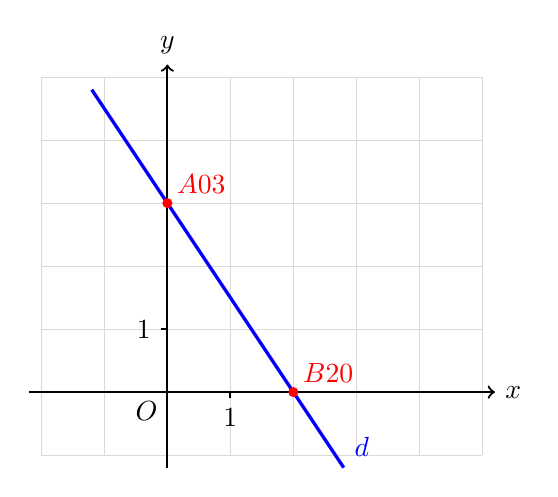
\begin{tikzpicture}[scale=0.8]
			\draw[step=1cm,gray!30,very thin] (-2,-1) grid (5,5);
			\draw[thick,->] (-2.2,0) -- (5.2,0) node[right] {$x$};
			\draw[thick,->] (0,-1.2) -- (0,5.2) node[above] {$y$};
			\node[below left] at (0,0) {$O$};
			\draw[thick] (1,0) -- (1,-0.1) node[below] {$1$};
			\draw[thick] (0,1) -- (-0.1,1) node[left] {$1$};
			\draw[line width=1.2pt, blue, domain=-1.2:2.8] plot (\x, {-1.5*\x + 3}) node[above right] {$d$};
			\filldraw[red] (0,3) circle (2pt) node[above right] {$A\coordl{0}{3}$};
			\filldraw[red] (2,0) circle (2pt) node[above right] {$B\coordl{2}{0}$};
		\end{tikzpicture}
	\end{center}
	\begin{remarque}
		Dans cet exemple, nous avons choisi $x = 0$ puis $y = 0$ car la valeur $0$ simplifie grandement les calculs.

		Il est tout à fait possible de choisir n'importe quelle autre valeur pour $x$ (ou pour $y$) pour trouver les points de la droite.
	\end{remarque}
\end{ex}

\begin{prop}[Vecteur directeur et coefficients]
	Soit $(d)$ une droite d'équation cartésienne $ax + by + c = 0$. Le vecteur $\vec{u}\coord{-b}{a}$ est un vecteur directeur de $(d)$.

	\[
		(d) : ax + by + c = 0 \iff \vec{u}\coord{-b}{a} \text{ vecteur directeur de } (d)
	\]
\end{prop}

\begin{ex}
	Soit $(d)$ la droite d'équation cartésienne $2x + 3y - 9 = 0$.

	Ici, $a = 2$, $b = 3$ et $c = -9$.

	D'après la propriété, un vecteur directeur de $(d)$ est :
	\[
		\vec{u}\coord{-b}{a} \iff \vec{u}\coord{-3}{2}
	\]

	Pour tracer la droite $(d)$, déterminons deux points à l'aide d'un point initial et du vecteur directeur :
	\begin{itemize}
		\item Pour $x = 0$ :

		      \begin{align*}
			      2\times 0 + 3y - 9 = 0 & \eqv 3y = 9 \\ &\eqv y = 3
		      \end{align*}

		      Donc $A\coordl{0}{3} \in (d)$.
		\item En partant du point $A\coordl{0}{3}$, on applique le vecteur directeur $\vec{u}\coord{-3}{2}$ (déplacement de $-3$ en abscisse et de $+2$ en ordonnée) pour obtenir le point $B\coordl{-3}{5} \in (d)$.
	\end{itemize}

	\begin{center}
		\begin{tikzpicture}[scale=0.85]
			\draw[step=1cm,gray!30,very thin] (-4,-1) grid (6,6);
			\draw[thick,->] (-4.2,0) -- (6.2,0) node[right] {$x$};
			\draw[thick,->] (0,-1.2) -- (0,6.2) node[above] {$y$};
			\node[below left] at (0,0) {$O$};
			\draw[thick] (1,0) -- (1,-0.1) node[below] {$1$};
			\draw[thick] (0,1) -- (-0.1,1) node[left] {$1$};
			\draw[line width=1pt, gray, domain=-4:6] plot (\x, {-2/3*\x + 3}) node[above right] {$(d)$};
			\draw[line width=1.5pt, black, -Stealth] (5,3) -- (2,5) node[midway, above right=-4mm,fill=white] {$\vec{u}\coord{-3}{2}$};
			\draw[line width=1.5pt, black, -Stealth] (5,3) -- (2,5);
			\draw[line width=1.5pt, black, -Stealth] (0,3) -- (-3,5);
			\filldraw[black] (0,3) circle (2.2pt) node[above right] {$A\coordl{0}{3}$};
			\filldraw[black] (-3,5) circle (2.2pt) node[below left, fill=white] {$B\coordl{-3}{5}$};
			\filldraw[black] (-3,5) circle (2.2pt);
			\draw[dashed, black!70, thick] (0,3) -- (-3,3) node[midway, below] {$-3$};
			\draw[dashed, black!70, thick] (-3,3) -- (-3,5) node[midway, left] {$+2$};
		\end{tikzpicture}
	\end{center}
\end{ex}

\begin{demo}
	Soit $A\coordl{x_0}{y_0}$ un point fixé de la droite $d$ et $\vec{u}\coord{\alpha}{\beta}$ un vecteur directeur non nul de $d$. Un point $M\coordl{x}{y}$ appartient à la droite $d$ si et seulement si les vecteurs $\vec{AM}\coord{x - x_0}{y - y_0}$ et $\vec{u}\coord{\alpha}{\beta}$ sont colinéaires.

	Or, la colinéarité équivaut à la nullité du déterminant :
	\begin{align*}
		M \in d & \eqv \determinant{x - x_0                                                        & \alpha \\ y - y_0 & \beta} = 0 \\
		        & \eqv \beta(x - x_0) - \alpha(y - y_0) = 0                                                 \\
		        & \eqv \boxed{\beta} x + \boxed{- \alpha} y + \boxed{(\alpha y_0 - \beta x_0)} = 0
	\end{align*}

	En posant $a = \beta$, $b = -\alpha$ et $c = \alpha y_0 - \beta x_0$, l'équation s'écrit bien sous la forme $ax + by + c = 0$.

	Puisque $\vec{u} \neq \vec{0}$, le couple $(\alpha\,;\,\beta) \neq (0\,;\,0)$, ce qui garantit $(a\,;\,b) \neq (0\,;\,0)$.

	De plus, les coordonnées du vecteur directeur $\vec{u}$ s'expriment sous la forme :
	\[
		\coord{\alpha}{\beta} = \coord{-b}{a}
	\]
\end{demo}

\begin{remarque}
	L'équation cartésienne d'une droite n'est pas unique.

	Si $ax + by + c = 0$ est une équation cartésienne de $d$, alors pour tout réel $k \neq 0$, $kax + kby + kc = 0$ est aussi une équation cartésienne de $d$.
\end{remarque}

\begin{methode}[Déterminer une équation cartésienne par le déterminant]
	Pour déterminer une équation cartésienne de $d$ connaissant $A\coordl{x_A}{y_A}$ et un vecteur directeur $\vec{u}\coord{u_x}{u_y}$ :

	\begin{enumerate}
		\item Soit $M\coordl{x}{y}$ un point quelconque du plan. Exprimer les coordonnées de $\vec{AM}\coord{x - x_A}{y - y_A}$.
		\item Écrire la condition de colinéarité : $\det\pa{\vec{AM};\vec{u}} = 0$.
		\item Développer et réduire l'expression pour obtenir la forme $ax + by + c = 0$.
	\end{enumerate}
\end{methode}

\begin{exemple}
	Déterminer une équation cartésienne de la droite $d$ passant par $A\coordl{3}{-1}$ et dirigée par le vecteur $\vec{u}\coord{-2}{5}$.

	\begin{correction}
		Soit $M\coordl{x}{y}$ un point du plan. On a $\vec{AM}\coord{x - 3}{y + 1}$.

		\begin{align*}
			M \in d & \eqv \det\pa{\vec{AM};\vec{u}} = 0                          \\
			        & \eqv \determinant{x - 3                                & -2 \\ y + 1 & 5} = 0 \\
			        & \eqv 5(x - 3) - (-2)(y + 1) = 0                             \\
			        & \eqv 5x - 15 + 2y + 2 = 0 \qquad \eqv 5x + 2y - 13 = 0
		\end{align*}

		Une équation cartésienne de la droite $d$ est $5x + 2y - 13 = 0$.
		
		\begin{center}
			\begin{tikzpicture}[scale=0.65]
				\draw[step=1cm,gray!30,very thin] (-1,-5) grid (6,7);
				\draw[thick,->] (-1,0) -- (6,0) node[above] {$x$};
				\draw[thick,->] (0,-5) -- (0,7) node[right] {$y$};
				\node[below left] at (0,0) {$O$};
				\draw[thick] (1,0) -- (1,-0.1) node[below] {$1$};
				\draw[thick] (0,1) -- (-0.1,1) node[left] {$1$};
				\coordinate (A) at (3,-1);
				\coordinate (M) at (4,-3.5);
				\filldraw[blue!70!black] (M) circle (2.2pt) node[right, fill=white] {$M\coordl{x}{y}$};
				\draw[line width=1.2pt, blue, domain=-0.2:4.6] plot (\x, {-2.5*\x + 6.5}) node[above right] {$d$};
				\filldraw[red] (A) circle (2.2pt) node[right, fill=white] {$A\coordl{3}{-1}$};
				\draw[line width=1.5pt, red, -Stealth] (3,-1) -- (1,4) node[midway, above,sloped, fill=white] {$\vec{u}\coord{-2}{5}$};
				\draw[line width=1.5pt, red, -Stealth] (3,-1) -- (1,4);
				\draw[line width=1.2pt, -Stealth] (A) -- (M) node[midway, below, sloped] {$\vec{AM}$};
				\draw[line width=1.2pt, -Stealth] (A) -- (M);
				\filldraw[red] (A) circle (2.2pt);
				\filldraw[blue!70!black] (M) circle (2.2pt);
				\draw[dashed, red!70, thick] (3,-1) -- (1,-1) node[midway, below] {$-2$};
				\draw[dashed, red!70, thick] (1,-1) -- (1,4) node[midway, left] {$+5$};
			\end{tikzpicture}
		\end{center}
	\end{correction}
\end{exemple}

\begin{methode}[Tracer une droite à partir de son équation cartésienne]
	Pour tracer la droite $d$ d'équation $ax + by + c = 0$ :

	\begin{enumerate}
		\item Déterminer un vecteur directeur $\vec{u}\coord{-b}{a}$.
		\item Choisir une valeur simple pour $x$ (par exemple $x = 0$), calculer l'ordonnée $y$ correspondante pour obtenir un premier point $A$.

		      Si les calculs mènent à des fractions, choisir un autre entier pour $x$.
		\item Placer le point $A$ puis appliquer le vecteur $\vec{u}$ pour tracer la droite.
	\end{enumerate}
\end{methode}

\begin{ex}
	Soit $d$ la droite d'équation cartésienne $2x + 3y - 6 = 0$.

	\begin{enumerate}
		\item \textbf{Vecteur directeur :} Ici, $a = 2$, $b = 3$ et $c = -6$.

		      Un vecteur directeur est $\vec{u}\coord{-b}{a} = \coord{-3}{2}$, ou son opposé $\vec{v}\coord{3}{-2}$.

		\item \textbf{Recherche d'un point :} Pour $x = 0$, on a :
		      \[
			      2 \times 0 + 3y - 6 = 0 \eqv 3y = 6 \eqv y = 2
		      \]
		      Le point $A\coordl{0}{2}$ appartient donc à la droite $d$.

		\item \textbf{Tracé de la droite :} On place le point $A\coordl{0}{2}$, puis à partir de $A$, on applique le vecteur $\vec{v}\coord{3}{-2}$ ($+3$ en abscisse, $-2$ en ordonnée) pour placer un second point $B\coordl{3}{0}$ et tracer la droite $d$.
	\end{enumerate}
% TODO: illustrationà revoir	
	\begin{center}
		\begin{tikzpicture}[scale=0.8]
			\draw[step=1cm,gray!30,very thin] (-2,-2) grid (6,4);
			\draw[thick,->] (-2.2,0) -- (6.2,0) node[right] {$x$};
			\draw[thick,->] (0,-2.2) -- (0,4.2) node[above] {$y$};
			\node[below left] at (0,0) {$O$};
			\draw[thick] (1,0) -- (1,-0.1) node[below] {$1$};
			\draw[thick] (0,1) -- (-0.1,1) node[left] {$1$};

			% Droite 2x + 3y - 6 = 0 => y = -2/3 x + 2
			\draw[line width=1.2pt, blue, domain=-2:6] plot (\x, {-2/3*\x + 2}) node[above right] {$d$};

			% Vecteur v applique en A(0,2) vers B(3,0)
			\draw[line width=1.5pt, red, -Stealth] (0,2) -- (3,0) node[midway, above right] {$\vec{v}\coord{3}{-2}$};

			% Points A et B
			\filldraw[red] (0,2) circle (2.2pt) node[above right] {$A\coordl{0}{2}$};
			\filldraw[red] (3,0) circle (2.2pt) node[above right] {$B\coordl{3}{0}$};

			% Composantes du vecteur
			\draw[dashed, red!70, thick] (0,2) -- (3,2) node[midway, above] {$+3$};
			\draw[dashed, red!70, thick] (3,2) -- (3,0) node[midway, right] {$-2$};
		\end{tikzpicture}
	\end{center}
\end{ex}
\subsection{Position relative et critère de parallélisme}

\begin{prop}[Parallélisme via équations cartésiennes]
	Soient deux droites $d$ et $d'$ d'équations cartésiennes respectives $ax + by + c = 0$ et $a'x + b'y + c' = 0$.
	\begin{itemize}
		\item $d$ et $d'$ sont parallèles si et seulement si leurs vecteurs directeurs $\vec{u}\coord{-b}{a}$ et $\vec{u'}\coord{-b'}{a'}$ sont colinéaires, c'est-à-dire :
		      \[
			      \determinant{\vec{u} & \vec{u'}} = 0 \eqv ab' - a'b = 0
		      \]
		\item $d$ et $d'$ sont sécantes si et seulement si $ab' - a'b \neq 0$.
	\end{itemize}
\end{prop}

\begin{exemple}
	Démontrer que les droites $d_1 : 3x - 2y + 5 = 0$ et $d_2 : -6x + 4y + 1 = 0$ sont parallèles.

	\begin{correction}
		Un vecteur directeur de $d_1$ est $\vec{u_1}\coord{2}{3}$. Un vecteur directeur de $d_2$ est $\vec{u_2}\coord{-4}{-6}$.

		Calculons leur déterminant :
		\[
			\determinant{\vec{u_1} & \vec{u_2}} = \determinant{2 & -4 \\ 3 & -6} = 2 \times (-6) - 3 \times (-4) = -12 + 12 = 0
		\]
		Les vecteurs $\vec{u_1}$ et $\vec{u_2}$ sont colinéaires, donc les droites $d_1$ et $d_2$ sont parallèles.
	\end{correction}
\end{exemple}

\section{Équation réduite et pente d'une droite}

\subsection{Équation réduite d'une droite}

\begin{prop}[Équation réduite]
	Toute droite $d$ du plan admet une unique équation, appelée \textbf{équation réduite}, de l'une des deux formes suivantes :
	\begin{itemize}
		\item Si $d$ est parallèle à l'axe des ordonnées, son équation réduite est de la forme :
		      \[
			      x = k \quad (k \in \R)
		      \]
		\item Si $d$ n'est pas parallèle à l'axe des ordonnées, son équation réduite est de la forme :
		      \[
			      y = mx + p \quad (m, p \in \R)
		      \]
	\end{itemize}
\end{prop}

\begin{definition}[Vocabulaire]
	Pour une droite $d$ d'équation réduite $y = mx + p$ :
	\begin{itemize}
		\item Le réel $m$ est appelé la \textbf{pente} ou le \textbf{coefficient directeur} de la droite $d$.
		\item Le réel $p$ est appelé l'\textbf{ordonnée à l'origine} de la droite $d$.
	\end{itemize}
\end{definition}

\begin{remarque}
	Une droite non parallèle à l'axe des ordonnées d'équation $y = mx + p$ admet pour vecteur directeur le vecteur $\vec{u}\coord{1}{m}$.
\end{remarque}

\begin{methode}[Passer de l'équation cartésienne à l'équation réduite]
	Soit la droite $d$ d'équation cartésienne $ax + by + c = 0$.
	\begin{itemize}
		\item Si $b = 0$, alors $a \neq 0$. L'équation s'écrit $ax + c = 0$, soit $x = -\frac{c}{a}$. C'est une droite parallèle à l'axe des ordonnées.
		\item Si $b \neq 0$, on isole $y$ dans l'équation :
		      \[
			      by = -ax - c \eqv y = -\frac{a}{b}x - \frac{c}{b}
		      \]
		      On identifie alors la pente $m = -\frac{a}{b}$ et l'ordonnée à l'origine $p = -\frac{c}{b}$.
	\end{itemize}
\end{methode}

\subsection{Calcul du coefficient directeur}

\begin{prop}[Calcul de la pente par deux points]
	Soient $A\coordl{x_A}{y_A}$ et $B\coordl{x_B}{y_B}$ deux points distincts d'une droite $d$. Si $x_A \neq x_B$, la droite $d$ n'est pas parallèle à l'axe des ordonnées et son coefficient directeur $m$ est donné par la formule :
	\[
		m = \frac{y_B - y_A}{x_B - x_A}
	\]
\end{prop}

\begin{exemple}
	Déterminer l'équation réduite de la droite $d$ passant par les points $A\coordl{2}{5}$ et $B\coordl{-1}{11}$.

	\begin{correction}
		Comme $x_A = 2$ et $x_B = -1$, on a $x_A \neq x_B$. La droite $d$ admet donc une équation réduite de la forme $y = mx + p$.
		\begin{enumerate}
			\item Calcul du coefficient directeur $m$ :
			      \[
				      m = \frac{y_B - y_A}{x_B - x_A} = \frac{11 - 5}{-1 - 2} = \frac{6}{-3} = -2
			      \]
			      L'équation s'écrit donc $y = -2x + p$.
			\item Calcul de l'ordonnée à l'origine $p$ : Le point $A\coordl{2}{5}$ appartient à $d$, ses coordonnées vérifient son équation :
			      \[
				      5 = -2 \times 2 + p \eqv 5 = -4 + p \eqv p = 9
			      \]
		\end{enumerate}
		L'équation réduite de $d$ est $y = -2x + 9$.
	\end{correction}
\end{exemple}

\subsection{Parallélisme avec les équations réduites}

\begin{prop}[Critère de parallélisme]
	Soient deux droites $d$ et $d'$ d'équations réduites respectives $y = mx + p$ et $y = m'x + p'$.
	\begin{itemize}
		\item $d$ et $d'$ sont parallèles si et seulement si elles ont le même coefficient directeur :
		      \[
			      d \parallel d' \eqv m = m'
		      \]
		\item $d$ et $d'$ sont sécantes si et seulement si leurs coefficients directeurs sont différents ($m \neq m'$).
	\end{itemize}
\end{prop}

\section{Exercices types}

\begin{exercice}
	Soient $A\coordl{-2}{1}$, $B\coordl{1}{3}$ et $C\coordl{4}{5}$ trois points du plan.
	\begin{enumerate}
		\item Déterminer une équation cartésienne de la droite $(AB)$.
		\item Les points $A$, $B$ et $C$ sont-ils alignés ?
	\end{enumerate}
\end{exercice}

\begin{correction}
	\nline
	\begin{enumerate}
		\item Le vecteur $\vec{AB}$ a pour coordonnées $\coord{1 - (-2)}{3 - 1} = \coord{3}{2}$. Soit $M\coordl{x}{y}$ un point du plan.
		      \begin{align*}
			      M \in (AB) & \eqv \determinant{\vec{AM}   & \vec{AB}} = 0 \\
			                 & \eqv \determinant{x + 2      & 3             \\ y - 1 & 2} = 0 \\
			                 & \eqv 2(x + 2) - 3(y - 1) = 0                 \\
			                 & \eqv 2x + 4 - 3y + 3 = 0                     \\
			                 & \eqv 2x - 3y + 7 = 0
		      \end{align*}
		      Une équation cartésienne de $(AB)$ est $2x - 3y + 7 = 0$.

		\item Testons si les coordonnées du point $C\coordl{4}{5}$ vérifient cette équation :
		      \[
			      2x_C - 3y_C + 7 = 2(4) - 3(5) + 7 = 8 - 15 + 7 = 0
		      \]
		      Les coordonnées de $C$ vérifient l'équation de la droite $(AB)$, donc $C \in (AB)$. Par conséquent, les points $A$, $B$ et $C$ sont alignés.
	\end{enumerate}
\end{correction}

\begin{exercice}
	On considère les droites $d_1 : 4x - 6y + 3 = 0$ et $d_2 : y = \frac{2}{3}x - 5$.
	\begin{enumerate}
		\item Déterminer l'équation réduite de $d_1$.
		\item Étudier la position relative de $d_1$ et $d_2$.
	\end{enumerate}
\end{exercice}

\begin{correction}
	\nline
	\begin{enumerate}
		\item Pour la droite $d_1$, isolons $y$ :
		      \[
			      4x - 6y + 3 = 0 \eqv 6y = 4x + 3 \eqv y = \frac{4}{6}x + \frac{3}{6} \eqv y = \frac{2}{3}x + \frac{1}{2}
		      \]
		      L'équation réduite de $d_1$ est $y = \frac{2}{3}x + \frac{1}{2}$.

		\item Le coefficient directeur de $d_1$ est $m_1 = \frac{2}{3}$. Le coefficient directeur de $d_2$ est $m_2 = \frac{2}{3}$. Puisque $m_1 = m_2$, les droites $d_1$ et $d_2$ sont parallèles. De plus, leurs ordonnées à l'origine sont différentes ($\frac{1}{2} \neq -5$), donc $d_1$ et $d_2$ sont strictement parallèles.
	\end{enumerate}
\end{correction}

\ifpoly
	\maketitle
	\tableofcontents
	\chapter{Algorithmes et programmation}

\section{Variable, affectation et types de données}

\begin{defin}[Variable et affectation]
	En programmation, une \textbf{variable} est un espace mémoire nommé servant à stocker une donnée.

	L'\textbf{affectation} est l'opération qui consiste à attribuer une valeur à une variable.

	En Python, elle est réalisée à l'aide du symbole \lstinline|=|.
\end{defin}

\begin{remarque}
	Dans une instruction d'affectation ~\lstinline|x = expression|~, l'évaluation de l'expression située à droite du ~\lstinline|=|~ est effectuée en premier, puis le résultat est stocké dans la variable ~\lstinline|x|.
\end{remarque}

\begin{ex}
	\nline
	\begin{lstlisting}
a=5
b=a+2
a=a+1
\end{lstlisting}

	\begin{itemize}
		\item \lstinline|a=5| : affecte la valeur entière $5$ à la variable \lstinline|a|.
		\item \lstinline|b=a+2| : évalue $5 + 2$, puis affecte la valeur $7$ à la variable \lstinline|b|.
		\item \lstinline|a=a+1| : augmente de $1$ la valeur contenue dans \lstinline|a| (opération d'incrémentation).
	\end{itemize}
\end{ex}

\begin{prop}[Principaux types de données en Python]
	En Python, chaque variable possède un type déterminé par la valeur qu'elle contient :
	\begin{itemize}
		\item \textbf{Entiers} (\lstinline|int|) : nombres entiers relatifs (ex. : \lstinline|3|, \lstinline|-12|).
		\item \textbf{Flottants} (\lstinline|float|) : nombres décimaux (ex. : \lstinline|3.14|, \lstinline|-0.5|).
		\item \textbf{Chaînes de caractères} (\lstinline|str|) : suites de caractères délimitées par des guillemets (ex. : \lstinline|"Maths"|, \lstinline|'Python'|).
		\item \textbf{Booléens} (\lstinline|bool|) : valeurs de vérité, soit \lstinline|True| (Vrai), soit \lstinline|False| (Faux).
	\end{itemize}
\end{prop}

\begin{attention}
	Le séparateur décimal en Python est le point \lstinline|.| et non la virgule \lstinline|,|.

	De plus, la chaîne de caractères \lstinline|"5"| de type \lstinline|str| est différente du nombre entier \lstinline|5| de type \lstinline|int|.
\end{attention}

\begin{prop}[Opérateurs arithmétiques]
	Soient \lstinline|a| et \lstinline|b| deux variables numériques. Les principaux opérateurs sont :
	\begin{multicols}{2}
		\begin{itemize}
			\item \lstinline|a + b| : Addition
			\item \lstinline|a - b| : Soustraction
			\item \lstinline|a * b| : Multiplication
			\item \lstinline|a / b| : Division exacte (résultat \lstinline|float|)
			\item \lstinline|a // b| : Quotient de la division entière
			\item \lstinline|a % b| : Reste de la division entière (modulo)
			\item \lstinline|a ** b| : Puissance ($a^b$)
		\end{itemize}
	\end{multicols}
\end{prop}

\newpage

\begin{methode}[Échanger les valeurs de deux variables]
	Pour échanger les contenus de deux variables \lstinline|a| et \lstinline|b|, il est nécessaire de passer par une variable temporaire \lstinline|temp| pour ne pas perdre de donnée, ou d'utiliser l'affectation simultanée propre à Python.

	\begin{correction}
		\nline
		{
			\setlength{\columnseprule}{0.6pt}
			\begin{multicols}{2}
				\noindent\textbf{Méthode avec variable temporaire :}
				\begin{lstlisting}[language=Python]
temp = a
a = b
b = temp
\end{lstlisting}
				\columnbreak
				\noindent\textbf{Méthode propre à Python :}
				\begin{lstlisting}[language=Python]
a, b = b, a
	
	
\end{lstlisting}
			\end{multicols}
		}
	\end{correction}
\end{methode}

\section{Structure conditionnelle}

\begin{defin}[Structure conditionnelle]
	Une \textbf{structure conditionnelle} permet d'exécuter un bloc d'instructions uniquement si une condition donnée (une expression booléenne) est vérifiée.
\end{defin}

\begin{prop}[Opérateurs de comparaison]
	Les conditions s'expriment à l'aide des opérateurs de comparaison suivants :
	\begin{multicols}{3}
		\begin{itemize}
			\item \lstinline|==| : Égal à
			\item \lstinline|!=| : Différent de
			\item \lstinline|<| : Strictement inférieur
			\item \lstinline|>| : Strictement supérieur
			\item \lstinline|<=| : Inférieur ou égal
			\item \lstinline|>=| : Supérieur ou égal
		\end{itemize}
	\end{multicols}
\end{prop}

\begin{attention}
	Il ne faut pas confondre le symbole d'affectation \lstinline|=| avec le test d'égalité \lstinline|==|.
\end{attention}

\begin{defin}[Syntaxe des blocs \lstinline|if / elif / else|]
	En Python, les blocs d'instructions sont délimités par des deux-points \lstinline|:| et par l'\textbf{indentation} (décalage vers la droite systématique d'une tabulations ou $4$ espaces).

	\begin{lstlisting}[language=Python]
if condition_1:
    # Instructions si condition_1 est vraie
elif condition_2:
    # Instructions si condition_1 est fausse et condition_2 vraie
else:
    # Instructions si aucune condition n'est vraie
\end{lstlisting}
\end{defin}

\begin{methode}[Mise en œuvre d'une structure conditionnelle]
	On souhaite déterminer si un nombre réel $x$ appartient à l'intervalle $\intff{2}{5}$.

	\begin{correction}
		\nline
		\begin{lstlisting}[language=Python]
if x >= 2 and x <= 5:
    print("x appartient a l'intervalle [2 ; 5]")
else:
    print("x n'appartient pas a l'intervalle [2 ; 5]")
\end{lstlisting}
	\end{correction}
\end{methode}

\begin{remarque}[Opérateurs logiques]
	Les conditions complexes peuvent être combinées à l'aide des opérateurs logiques :
	\begin{itemize}
		\item \lstinline|and| (ET) : vrai si toutes les conditions sont vraies simultanément.
		\item \lstinline|or| (OU) : vrai si au moins l'une des conditions est vraie.
		\item \lstinline|not| (NON) : inverse l'état logique d'une condition.
	\end{itemize}
\end{remarque}


\section{Structures itératives (Boucles)}

\begin{defin}[Boucle bornée \texttt{for}]
	Une \textbf{boucle bornée} répète un bloc d'instructions un nombre déterminé à l'avance de fois.

	En Python, elle s'écrit avec la commande \lstinline|for| combinée avec \lstinline|range()|.
\end{defin}

\begin{prop}[Fonction \texttt{range}]
	La fonction \lstinline|range()| génère une séquence d'entiers :
	\begin{itemize}
		\item \lstinline|range(n)| génère les $n$ entiers de $0$ à $n-1$.
		\item \lstinline|range(a, b)| génère les entiers de $a$ à $b-1$.
		\item \lstinline|range(a, b, k)| génère les entiers de $a$ à $b-1$ par pas de $k$.
	\end{itemize}
\end{prop}

\begin{ex}
	Le code suivant calcule la somme $S = 1 + 2 + 3 + \dots + 10$ :
	\begin{lstlisting}[language=Python]
S = 0
for i in range(1, 11):
    S = S + i
print(S)
\end{lstlisting}
\end{ex}

\begin{defin}[Boucle non bornée \texttt{while}]
	Une \textbf{boucle non bornée} répète un bloc d'instructions tant qu'une condition reste vraie.

	Le nombre d'itérations n'est pas connu à l'avance.
	\begin{lstlisting}[language=Python]
while condition:
    # Instructions a repeter
\end{lstlisting}
\end{defin}

\begin{attention}[Risque de boucle infinie]
	Dans une boucle \lstinline|while|, la condition doit obligatoirement devenir fausse à un moment donné.

	Si la variable de contrôle n'est pas modifiée dans le corps de la boucle, le programme boucle indéfiniment.
\end{attention}

\begin{methode}[Utiliser une boucle \lstinline|while|]
	On place la somme de $1000$ € sur un compte à un taux d'intérêts annuel de $5\,\%$.

	On souhaite déterminer au bout de combien d'années le capital dépassera $1500$ €.

	\begin{correction}
		\nline
		\begin{lstlisting}[language=Python]
capital = 1000
annees = 0
while capital <= 1500:
    capital = capital * 1.05
    annees = annees + 1
print("Nombre d'annees :", annees)
\end{lstlisting}
	\end{correction}
\end{methode}

\section{Fonctions et modularité}

\begin{defin}[Fonction]
	En programmation, une \textbf{fonction} est un bloc d'instructions nommé qui effectue une tâche précise.

	Elle peut recevoir des paramètres d'entrée (arguments) et renvoyer un résultat à l'aide du mot-clé \lstinline|return|.
\end{defin}

\begin{defin}[Syntaxe d'une fonction]
	\nline
	\begin{lstlisting}[language=Python]
def nom_de_la_fonction(parametre1, parametre2):
    # Bloc d'instructions
    resultat = ...
    return resultat
\end{lstlisting}
\end{defin}

\begin{methode}[Définir et appeler une fonction mathématique]
	Soit la fonction mathématique $f: x \mapsto 3x^2 - 5x + 2$.

	Créer une fonction Python nommée \lstinline|f| prenant en paramètre un nombre \lstinline|x| et renvoyant son image par $f$.

	\begin{correction}
		\nline
		\begin{lstlisting}[language=Python]
def f(x):
    y = 3 * x**2 - 5 * x + 2
    return y

# Appel de la fonction pour x = 4
image = f(4)
print(image)
\end{lstlisting}
	\end{correction}
\end{methode}

\begin{remarque}
	L'instruction \lstinline|return| interrompt immédiatement l'exécution de la fonction et renvoie la valeur spécifiée. Si une fonction ne contient pas d'instruction \lstinline|return|, elle renvoie la valeur \lstinline|None|.
\end{remarque}

\begin{methode}[Algorithme de calcul de distance dans le plan]
	Créer une fonction \lstinline|distance(xA, yA, xB, yB)| qui renvoie la distance entre deux points $A(x_A, y_A)$ et $B(x_B, y_B)$ dans un repère orthonormé :
	\[
		AB = \sqrt{(x_B - x_A)^2 + (y_B - y_A)^2}
	\]

	\begin{correction}
		\nline
		\begin{lstlisting}[language=Python]
from math import sqrt

def distance(xA, yA, xB, yB):
    d = sqrt((xB - xA)**2 + (yB - yA)**2)
    return d
\end{lstlisting}
	\end{correction}
\end{methode}

	\newpage

\section{Exercices}
 {
  \small
  \setlength{\columnseprule}{0.6pt}
  \begin{multicols}{2}

	  \begin{exo}[Analyse d'affectations]
		  Soient les instructions suivantes exécutées successivement :

		  \begin{lstlisting}
a = 3
b = 7
a = a + b
b = a - b
a = a - b
\end{lstlisting}

		  Quelles sont les valeurs finales des variables \lstinline|a| et \lstinline|b| ?
	  \end{exo}

	  \begin{exo}[Calculs arithmétiques]
		  Soient \lstinline|x = 17| et \lstinline|y = 5|. Donner le résultat et le type des expressions suivantes :
		  \begin{enumerate}[label=\alph*)]
			  \item \lstinline|x / y|
			  \item \lstinline|x // y|
			  \item \lstinline|x % y|
			  \item \lstinline|x ** 2|
		  \end{enumerate}
	  \end{exo}

	  \begin{exo}{}
		  Expliquer de façon claire et concise ce que fait le programme suivant.

		  \begin{lstlisting}
a=int(input("Entrez un entier"))
b=a
a=a*b
print(a)
\end{lstlisting}
	  \end{exo}

	  \begin{exo}{}
		  Qu'affichera le programme suivant ?

		  \begin{lstlisting}
a=1
b=2
c=a+b
a=b+c
b=c+a
print(b)
\end{lstlisting}
	  \end{exo}

	  \begin{exo}{}
		  Que fait le programme suivant ?

		  \begin{lstlisting}
a=int(input("Entrez un entier"))
b=a+a
a=a+b
print(a)
\end{lstlisting}
	  \end{exo}

	  \begin{exo}{}
		  Qu'affichera le programme suivant ?

		  \begin{lstlisting}
a=3
for i in range(1,1001):
    a=a+0.5
print(a)
\end{lstlisting}
	  \end{exo}

	  \vfill~\columnbreak

	  \begin{exo}{}
		  Que fait le programme suivant ?

		  \begin{lstlisting}
b=1
a=int(input("Entrez un nombre"))
for i in range(1,4):
    b=b*a
print(b)
\end{lstlisting}
	  \end{exo}

	  \begin{exo}{}
		  Compléter le programme suivant pour qu'il calcule la somme des inverses des entiers de $1$ à $1000$ :

		  \[
			  1 + \frac12 + \frac13 + \frac14 + \cdots + \frac1{1000}
		  \]

		  \begin{lstlisting}
somme=0
for i in range(1,1001):
    somme=somme+.........
print(somme)
\end{lstlisting}
	  \end{exo}

	  \begin{exo}{}
		  Écrivez un programme qui demande à l'utilisateur d'entrer un entier naturel non nul $n$ et qui affiche la factorielle de $n$.

		  La factorielle d'un entier $n$, notée $n!$, est le produit de tous les entiers de $1$ à $n$ inclus.

		  \[
			  5! = 1 \times 2 \times 3 \times 4 \times 5 = 120.
		  \]
	  \end{exo}

	  \begin{exo}{}
		  Que fait le programme suivant ?
		  {\footnotesize
		  \begin{lstlisting}
s=0
n=int(input("Entrez un entier > 0"))
for i in range(1,n+1):
    s=s+i
print(s)
\end{lstlisting}
		  }
	  \end{exo}

	  \begin{exo}{}
		  Que fait le programme suivant ?
		  {\footnotesize
		  \begin{lstlisting}
s=0
n=int(input("Entrez un entier > 0"))
p=int(input("Entrez-en un deuxième"))
for i in range(1,n+1):
    for j in range(1,p+1):
        s=s+1
print(s)
\end{lstlisting}
		  }
	  \end{exo}

	  \begin{exo}[Structure conditionnelle]
		  Écrire une fonction Python \lstinline|maximum(a, b)| qui prend deux nombres \lstinline|a| et \lstinline|b| en paramètres et renvoie le plus grand des deux sans utiliser la fonction native \lstinline|max()|.
	  \end{exo}

	  \vfill~\columnbreak

	  \begin{exo}{}
		  Le programme suivant tire au sort $20$ entiers entre $1$ et $100$ et affiche leur somme.

		  Modifiez-le pour qu'il affiche non plus la somme, mais le plus grand d'entre eux.

		  \begin{lstlisting}
from random import *

s=0
for i in range(1,21):
    a=randint(1,100)
    s=s+a
print(s)
\end{lstlisting}
	  \end{exo}

	  \begin{exo}{}
		  Modifiez le programme de l'exercice précédent pour qu'il affiche à la fin la moyenne des entiers tirés au sort.
	  \end{exo}

	  \begin{exo}[Boucle \texttt{while} et seuil]
		  On considère la suite de nombres définie par son premier terme $U_0 = 100$ et la relation $U_{n+1} = 0{,}8 U_n + 5$.

		  Écrire un programme Python déterminant le plus petit entier $n$ tel que $U_n < 30$.
	  \end{exo}

	  \begin{exo}{}
		  Qu'affichera le programme suivant ?

		  \begin{lstlisting}
a=30
n=1
while n<=a:
    n=2*n
print(n)
\end{lstlisting}
	  \end{exo}

	  \begin{exo}{}
		  Que fait le programme suivant ?

		  \begin{lstlisting}
a=input("Entrez un entier > 0")
a=int(a)
n=1
while n<=a:
    n=2*n
print(n)
\end{lstlisting}
	  \end{exo}

	  \begin{exo}{}
		  Un puits contient une hauteur d'eau de $10$ m. Chaque jour, son niveau diminue de $2$\%.

		  Compléter l'algorithme suivant pour qu'il calcule le nombre de jours qu'il faudra pour que le niveau descende en dessous de $1$ m.

		  \begin{lstlisting}
hauteur=10
nb_jours=0

while hauteur>1:
    nb_jours=............
    hauteur=............

print(nb_jours)
\end{lstlisting}
	  \end{exo}

	  \vfill~\columnbreak

	  \begin{exo}[Milieu et distance dans le plan]
		  On considère deux points $A(x_A, y_A)$ et $B(x_B, y_B)$ dans un repère orthonormé.

		  Écrire une fonction Python \lstinline|milieu(xA, yA, xB, yB)| qui renvoie les coordonnées $(x_I, y_I)$ du milieu $I$ du segment $[AB]$ sous forme d'un couple de valeurs.
	  \end{exo}

	  \begin{exo}{}
		  Qu'affichera le programme suivant ?

		  \begin{lstlisting}
def f(x):
    y=x**2+x+1
    return y

y=f(5)
print(y)
\end{lstlisting}
	  \end{exo}

	  \begin{exo}{}
		  Que fait la fonction suivante ?

		  \begin{lstlisting}
def ultime(a,b,c):
    if b>a:
        a=b
    if c>a:
        a=c
    return a
\end{lstlisting}
	  \end{exo}

	  \begin{exo}{}
		  Une urne contient $3$ boules blanches et $3$ boules noires. On effectue deux tirages avec remise.

		  Écrire une fonction qui simule la répétition à $n$ reprises de cette expérience et affiche le nombre de cas où le joueur a gagné (deux boules blanches).
	  \end{exo}

	  \begin{exo}{}
		  Dans le cadre d'un jeu de hasard, un joueur lance un dé.

		  S'il obtient \epsdice{5} ou $\epsdice{6}$, il gagne, sinon il perd.

		  La fonction suivante simule $n$ fois l'expérience et renvoie le nombre de cas où le joueur a gagné.

		  Modifier cette fonction afin qu'elle renvoie la \textbf{fréquence} des victoires.

		  Que se passe-t-il lorsque $n$ devient très grand ?
		  {\footnotesize
		  \begin{lstlisting}
from random import *

def echantillon(n):
    gagne=0
    for i in range(1,n+1):
        a=randint(1,6)
        if a>=5:
            gagne=gagne+1
    return gagne
\end{lstlisting}
		  }
	  \end{exo}
	  \vfill~

  \end{multicols}
 }

	\part{Nombres et calculs}
	\input{tex/2nde/fractions-puissances-racines}
	\chapter{Calcul algébrique}

\section{Somme et produit}

\begin{defin}
	Une \textbf{somme} est le résultat d'une addition. Les éléments que l'on additionne s'appellent des \textbf{termes}.

	Une \textbf{différence} est le résultat d'une soustraction. Tout comme la somme, elle est composée de \textbf{termes}.

	Un \textbf{produit} est le résultat d'une multiplication. Les éléments que l'on multiplie s'appellent des \textbf{facteurs}.

	Un \textbf{quotient} est le résultat d'une division. Il est composé d'un \textbf{numérateur} et d'un \textbf{dénominateur}.
\end{defin}

\begin{attention}
	Contrairement aux autres opérations, un quotient n'existe que si son dénominateur est \textbf{différent de zéro}.
	\[
		\frac{A}{B} \text{ n'existe que si } B \neq 0
	\]
\end{attention}

\begin{rem}
	Le produit et le quotient suivent la même règle :
	\begin{itemize}
		\item Signes identiques $\Rarr$ résultat positif ($+$).
		\item Signes contraires $\Rarr$ résultat négatif ($-$).
	\end{itemize}
\end{rem}

\begin{ex}
	\nline
	\begin{multicols}{3}
		\textbf{Sommes (ou différences)}
		\begin{itemize}
			\item $x - 3$
			\item $(2x + 4) + 3x$
			\item $(5 - x) - (9 + 9x)$
			\item $3 + (2 + 3x)(x - 2)$
		\end{itemize}

		\columnbreak

		\textbf{Produits de facteurs}
		\begin{itemize}
			\item $(6x + 1) \times (x - 1)$
			\item $2 \times (1 + 6x)$
			\item $(8 - x) \times (2 + x)$
			\item $(3 + 8x) \times (x - 8)^2$
		\end{itemize}

		\columnbreak

		\textbf{Quotients (num./dén.)}
		\begin{itemize}
			\item $\dfrac{x+3}{2}$
			\item $\dfrac{5}{x-1}$
			\item $\dfrac{3x^2+1}{2x-4}$
			      % \item $\dfrac{(x+1)(x-3)}{x^2+5}$
		\end{itemize}
	\end{multicols}
\end{ex}

\begin{defin}[Développer et factoriser]
	\nline
	\begin{itemize}
		\item \textbf{Développer} c'est transformer un produit (ou quotient) en une somme (ou différence).
		\item \textbf{Factoriser} c'est transformer une somme (ou différence) en un produit (ou quotient).
	\end{itemize}

	\begin{center}
		\begin{tikzpicture}[
			transform shape,
			block/.style={ rectangle, rounded corners=4pt, very thick, text centered, minimum width=11em, minimum height=3em, text width=10.5em, inner sep=3pt, font=\bfseries\large },
			block_sum/.style={ block, draw=red!75, fill=red!5 },
			block_prod/.style={block, draw=green!60!black, fill=green!5},
			arrow/.style={-{Stealth[scale=1.0]}, thick, shorten >=2pt, shorten <=2pt}
			]
			\node (product) [block_prod] {PRODUIT \\ (ou Quotient)};
			\node (sum) [block_sum, right=2.5cm of product] {SOMME \\ (ou Différence)};
			\draw [arrow, out=30, in=150] (product.north) to (sum.north);
			\path [decorate, decoration={text along path, text={D{é}velopper}, text align=center, raise=5pt}] (product.north) [out=30, in=150] to (sum.north);
			\draw [arrow, out=210, in=330] (sum.south) to (product.south);
			\path [decorate, decoration={text along path, text={Factoriser}, text align=center, raise=-15pt}] (product.south) [out=330, in=210] to (sum.south);
		\end{tikzpicture}
	\end{center}
\end{defin}

\newpage

\section{Développement}

\begin{prop}[Distributivité]
	Soient $a$, $b$ et $c$ trois nombres réels. On a :
	\begin{center}
		\begin{tikzpicture}[transform shape,arrow/.style={-{Stealth[scale=0.8]}, thick, color=blue!70!black},node distance=0.1cm ]
			\node (expr) {\Large $a(b + c) = ab + ac$};
			\path (expr.west) ++(0.35, 0.2) node (a_pos) {};
			\path (expr.west) ++(0.8, 0.2) node (b_pos) {};
			\path (expr.west) ++(1.5, 0.2) node (c_pos) {};
			\draw [arrow] (a_pos.center) to[out=85, in=95, distance=4mm] (b_pos.center);
			\draw [arrow] (a_pos.center) to[out=85, in=95, distance=7mm] (c_pos.center);
		\end{tikzpicture}
	\end{center}
\end{prop}

\begin{methode}[Développer une expression]
	Développer les expressions suivantes :
	\begin{multicols}{3}
		\begin{itemize}
			\item $A = 4(5 + x)$
			\item $B = 5(x - 2)$
			\item $C = (4x + 6) \times 3$
			\item $D = -6(-2x + 4)$
			\item $E = -x(2 - 3x)$
			\item $F = -(5 - x)$
		\end{itemize}
	\end{multicols}

	\begin{correction}
		\[
			\begin{array}{lll}%
				\def\arraystretch{1.3}%
				\begin{array}{rcl}%
					A & = & 4(5 + x) \\
					  & = & 20 + 4x  \\
				\end{array} \quad & \quad %
				\def\arraystretch{1.3}%
				\begin{array}{rcl}%
					B & = & 5(x - 2) \\
					  & = & 5x - 10  \\
				\end{array} \quad & \quad %
				\def\arraystretch{1.3}%
				\begin{array}{rcl}%
					C & = & (4x + 6) \times 3 \\
					  & = & 12x + 18          \\
				\end{array} \\&&\\%
				\def\arraystretch{1.3}%
				\begin{array}{rcl}%
					D & = & -6(-2x + 4) \\
					  & = & 12x - 24    \\
				\end{array} \quad & \quad %
				\def\arraystretch{1.3}%
				\begin{array}{rcl}%
					E & = & -x(2 - 3x) \\
					  & = & -2x + 3x^2 \\
				\end{array} \quad & \quad %
				\def\arraystretch{1.3}%
				\begin{array}{rcl}%
					F & = & -(5 - x) = -1(5 - x) \\
					  & = & -5 + x               \\
				\end{array}%
			\end{array}%
		\]
		\textit{Un signe $\pa{-}$ devant une parenthèse change les signes dans la parenthèse.}
	\end{correction}
\end{methode}

\begin{prop}[Double distributivité]
	Soient $a$, $b$, $c$ et $d$ quatre nombres réels. On a :
	\begin{center}
		\begin{tikzpicture}[transform shape,arrow_a/.style={-{Stealth[scale=0.8]}, thick, color=blue!70!black},arrow_b/.style={-{Stealth[scale=0.8]}, thick, color=red!70!black},node distance=0.1cm ]
			\node (expr) {\Large $(a + b)(c + d) = ac + ad + bc + bd$};
			\path (expr.west) ++(0.45, 0.2) node (a_top) {};
			\path (expr.west) ++(1.85, 0.2) node (c_top) {};
			\path (expr.west) ++(2.55, 0.2) node (d_top) {};
			\path (expr.west) ++(1.45, -0.2) node (b_bot) {};
			\path (expr.west) ++(1.85, -0.2) node (c_bot) {};
			\path (expr.west) ++(2.55, -0.2) node (d_bot) {};
			\draw [arrow_a] (a_top.center) to[out=80, in=100, distance=6mm] (c_top.center);
			\draw [arrow_a] (a_top.center) to[out=85, in=95, distance=11mm] (d_top.center);
			\draw [arrow_b] (b_bot.center) to[out=-80, in=-100, distance=5mm] (c_bot.center);
			\draw [arrow_b] (b_bot.center) to[out=-85, in=-95, distance=9mm] (d_bot.center);
		\end{tikzpicture}
	\end{center}
\end{prop}

\begin{methode}[Développer et réduire par double distributivité]
	Développer et réduire :
	\begin{multicols}{2}
		\begin{itemize}
			\item $A = (2x + 3)(x + 8)$
			\item $B = (-3 + x)(4 - 5x)$
			\item $C = 2(3 + x)(3 - 2x)$
			\item $D = 2x(1 - x) - (x - 3)(3x + 2)$
		\end{itemize}
	\end{multicols}

	\begin{correction}
		\[
			\begin{array}{ll}%
				\def\arraystretch{1.3}%
				\begin{array}{rcl}%
					A & = & (2x + 3)(x + 8)      \\
					  & = & 2x^2 + 16x + 3x + 24 \\
					  & = & 2x^2 + 19x + 24      \\
				\end{array}  \quad & \quad %
				\def\arraystretch{1.3}%
				\begin{array}{rcl}%
					B & = & (-3 + x)(4 - 5x)      \\
					  & = & -12 + 15x + 4x - 5x^2 \\
					  & = & -5x^2 + 19x - 12      \\
				\end{array} \\ & \\%
				\def\arraystretch{1.3}%
				\begin{array}{rcl}%
					C & = & 2(3 + x)(3 - 2x)      \\
					  & = & 2(9 - 6x + 3x - 2x^2) \\
					  & = & 2(-2x^2 - 3x + 9)     \\
					  & = & -4x^2 - 6x + 18       \\
				\end{array}  \quad & \quad %
				\def\arraystretch{1.3}%
				\begin{array}{rcl}%
					D & = & 2x(1 - x) - (x - 3)(3x + 2)      \\
					  & = & 2x - 2x^2 - (3x^2 + 2x - 9x - 6) \\
					  & = & 2x - 2x^2 - 3x^2 - 2x + 9x + 6   \\
					  & = & -5x^2 + 9x + 6                   \\
				\end{array}%
			\end{array}%
		\]
	\end{correction}
\end{methode}
\newpage

\section{Factorisation}

\begin{methode}[Factoriser par facteur commun (1)]
	Trouver le facteur commun, puis factoriser et réduire si possible :
	\begin{multicols}{3}
		\begin{itemize}
			\item $A = 3{,}5x - 4{,}2x + 2{,}1x$
			\item $B = 4t - 5tx + 3t$
			\item $C = 4x - 4y + 8$
			\item $D = x^2 + 3x - 5x^2$
			\item $E = 3t + 9u + 3$
			\item $F = 3x^2 - x$
		\end{itemize}
	\end{multicols}

	\begin{correction}
		\[
			\begin{array}{lll}%
				\def\arraystretch{1.3}%
				\begin{array}{rcl}%
					A & = & x(3{,}5 - 4{,}2 + 2{,}1) \\
					  & = & 1{,}4x
				\end{array}\quad & \quad %
				\def\arraystretch{1.3}%
				\begin{array}{rcl}%
					B & = & t(4 - 5x + 3) \\
					  & = & t(7 - 5x)
				\end{array}\quad & \quad %
				\def\arraystretch{1.3}%
				\begin{array}{rcl}%
					C & = & 4x - 4y + 4 \times 2 \\
					  & = & 4(x - y + 2)
				\end{array} \\~&~&~\\%
				\def\arraystretch{1.3}%
				\begin{array}{rcl}%
					D & = & x(x + 3 - 5x) \\
					  & = & x(-4x + 3)
				\end{array}\quad & \quad %
				\def\arraystretch{1.3}%
				\begin{array}{rcl}%
					E & = & 3(t + 3u + 1) \\
					  &   &               \\
				\end{array}\quad & \quad %
				\def\arraystretch{1.3}%
				\begin{array}{rcl}%
					F & = & x(3x - 1) \\
					  &   &           \\
				\end{array}%
			\end{array}%
		\]
	\end{correction}
\end{methode}

\begin{methode}[Factoriser par facteur commun (2)]
	Factoriser les expressions suivantes :
	\begin{multicols}{3}
		\begin{itemize}
			\item $A = 3(2 + 3x) - (5 + 2x)(2 + 3x)$
			\item $B = (2 - 5x)^2 - (2 - 5x)(1 + x)$
			\item $C = 5(1 - 2x) - (4 + 3x)(2x - 1)$
		\end{itemize}
	\end{multicols}

	\begin{correction}
		\[
			\begin{array}{ll}%
				\def\arraystretch{1.3}%
				\begin{array}{rcl}%
					A & =                                                 & 3(2 + 3x) - (5 + 2x)(2 + 3x) \\
					  & \multicolumn{2}{l}{\text{Facteur commun : } 2+3x}                                \\
					  & =                                                 & (2 + 3x)(3 - (5 + 2x))       \\
					  & =                                                 & (2 + 3x)(3 - 5 - 2x)         \\
					  & =                                                 & (2 + 3x)(-2 - 2x)            \\
					  &                                                   &                              \\
				\end{array} \quad & \quad %
				\def\arraystretch{1.3}%
				\begin{array}{rcl}%
					B & =                                                 & (2 - 5x)^2 - (2 - 5x)(1 + x)       \\
					  & =                                                 & (2 - 5x)(2 - 5x) - (2 - 5x)(1 + x) \\
					  & \multicolumn{2}{l}{\text{Facteur commun : } 2-5x}                                      \\
					  & =                                                 & (2 - 5x)((2 - 5x) - (1 + x))       \\
					  & =                                                 & (2 - 5x)(2 - 5x - 1 - x)           \\
					  & =                                                 & (2 - 5x)(1 - 6x)                   \\
				\end{array}%
			\end{array}%
		\]
		\ms
		On modifie l'écriture de $C$ pour faire apparaître un facteur commun : $(2x - 1) = -(1 - 2x)$
		\[
			\def\arraystretch{1.3}%
			\begin{array}{rcl}%
				C & =                                                 & 5(1 - 2x) - (4 + 3x)(2x - 1) \\
				  & =                                                 & 5(1 - 2x) + (4 + 3x)(1 - 2x) \\
				  & \multicolumn{2}{l}{\text{Facteur commun : } 1-2x}                                \\
				  & =                                                 & (1 - 2x)(5 + (4 + 3x))       \\
				  & =                                                 & (1 - 2x)(9 + 3x)             \\
			\end{array}%
		\]
	\end{correction}
\end{methode}

\newpage

\section{Identités remarquables}

\begin{prop}[Les trois identités remarquables]
	\[
		{(a+b)^2 = a^2 + 2ab + b^2} \qquad\qquad {(a-b)^2 = a^2 - 2ab + b^2} \qquad\qquad {(a+b)(a-b) = a^2 - b^2}
	\]
\end{prop}

\begin{ex}
	\[
		\begin{array}{ll}%
			\begin{array}{rcccccl}%
				(x + 3)^2 & = & x^2 & + & 2 \times x \times 3 & + & 3^2 \\
				          & = & x^2 & + & 6x                  & + & 9   \\
			\end{array}\qquad & \qquad %
			\begin{array}{rcccccl}%
				(x - 5)^2 & = & x^2 & - & 2 \times x \times 5 & + & 5^2 \\
				          & = & x^2 & - & 10x                 & + & 25  \\
			\end{array} \\ & \\%
			\begin{array}{rcccl}%
				(2x - 1)(2x + 1) & = & (2x)^2 & - & 1^2 \\
				                 & = & 4x^2   & - & 1
			\end{array}\qquad      & \qquad~    %
		\end{array}%
	\]
\end{ex}

\subsection{Développer avec les identités remarquables}

\begin{methode}[Développer avec les identités remarquables (1)]
	Développer et réduire éventuellement :
	\begin{multicols}{3}
		\begin{itemize}
			\item $A = (x + 3)^2$
			\item $B = (3x - 4)^2$
			\item $C = (x - 3)(x + 3)$
			\item $D = (2x + 3)(2x - 3)$
			\item $E = (4 - 3x)(3x + 4)$
		\end{itemize}
	\end{multicols}

	\begin{correction}
		\[
			\begin{array}{lll}%
				\def\arraystretch{1.3}%
				\begin{array}{rcl}%
					A & = & (x + 3)^2    \\
					  & = & x^2 + 6x + 9 \\
				\end{array} \quad & \quad %
				\def\arraystretch{1.3}%
				\begin{array}{rcl}%
					B & = & (3x - 4)^2      \\
					  & = & 9x^2 - 24x + 16 \\
				\end{array} \quad & \quad %
				\def\arraystretch{1.3}%
				\begin{array}{rcl}%
					C & = & (x - 3)(x + 3) \\
					  & = & x^2 - 9        \\
				\end{array} \\&\\%
				\def\arraystretch{1.3}%
				\begin{array}{rcl}%
					D & = & (2x + 3)(2x - 3) \\
					  & = & 4x^2 - 9         \\
					  &   &                  \\
				\end{array} \quad & \quad %
				\def\arraystretch{1.3}%
				\begin{array}{rcl}%
					E & = & (4 - 3x)(3x + 4) \\
					  & = & (4 - 3x)(4 + 3x) \\
					  & = & 16 - 9x^2        \\
				\end{array} & ~ %
			\end{array}%
		\]
	\end{correction}
\end{methode}

\begin{methode}[Développer avec les identités remarquables (2)]
	Développer et réduire :
	\begin{multicols}{3}
		\begin{itemize}
			\item $A = (2x - 3)^2 + (x + 5)(3 - x)$
			\item $B = (x - 3)(x + 3) - (4 - 3x)^2$
			\item $C = 2(x + 3) + (2x + 3)(2x - 3)$
		\end{itemize}
	\end{multicols}

	\begin{correction}
		\[
			\begin{array}{ll}%
				\def\arraystretch{1.3}%
				\begin{array}{rcl}%
					A & = & (2x - 3)^2 + (x + 5)(3 - x)         \\
					  & = & 4x^2 - 12x + 9 + 3x - x^2 + 15 - 5x \\
					  & = & 3x^2 - 14x + 24                     \\
					  &   &                                     \\
				\end{array} \quad & \quad %
				\def\arraystretch{1.3}%
				\begin{array}{rcl}%
					B & = & (x - 3)(x + 3) - (4 - 3x)^2 \\
					  & = & x^2 - 9 - (16 - 24x + 9x^2) \\
					  & = & x^2 - 9 - 16 + 24x - 9x^2   \\
					  & = & -8x^2 + 24x - 25            \\
				\end{array} \\%
				\def\arraystretch{1.3}%
				\begin{array}{rcl}%
					C & = & 2(x + 3) + (2x + 3)(2x - 3) \\
					  & = & 2x + 6 + 4x^2 - 9           \\
					  & = & 4x^2 + 2x - 3               \\
				\end{array}        \quad & \quad ~ %
			\end{array}%
		\]
	\end{correction}
\end{methode}

\newpage

\subsection{Factoriser avec les identités remarquables}

\begin{methode}[Factoriser avec les identités remarquables (1)]
	Factoriser :
	\begin{multicols}{3}
		\begin{itemize}
			\item $A = x^2 - 2x + 1$
			\item $B = 4x^2 + 12x + 9$
			\item $C = 9x^2 - 4$
			      % \item $D = 25 + 16x^2 - 40x$
			      % \item $E = 1 - 49x^2$
		\end{itemize}
	\end{multicols}

	\begin{correction}
		On identifie les termes $a^2$, $2ab$, $b^2$ des identités remarquables.
		\[
			\begin{array}{lll}%
				\def\arraystretch{1.3}%
				\begin{array}{rcl}%
					A & =                                                                            & x^2 - 2x + 1 \\
					  & \multicolumn{2}{l}{\quad\Rarr a=x,\ b=1 \quad\text{ (2}^\text{e}\text{ IR)}}                \\
					  & =                                                                            & (x - 1)^2    \\
					  &                                                                              &              \\
				\end{array}                         &                         %
				\def\arraystretch{1.3}%
				\begin{array}{rcl}%
					B & =                                                                              & 4x^2 + 12x + 9                      \\
					  & =                                                                              & (2x)^2 + 2 \times 2x \times 3 + 3^2 \\
					  & \multicolumn{2}{l}{\quad\Rarr a=2x,\ b=3 \quad\text{ (1}^\text{re}\text{ IR)}}                                       \\
					  & =                                                                              & (2x + 3)^2                          \\
				\end{array} & %
				\def\arraystretch{1.3}%
				\begin{array}{rcl}%
					C & =                                                                             & 9x^2 - 4         \\
					  & =                                                                             & (3x)^2 - 2^2     \\
					  & \multicolumn{2}{l}{\quad\Rarr a=3x,\ b=2 \quad\text{ (3}^\text{e}\text{ IR)}}                    \\
					  & =                                                                             & (3x - 2)(3x + 2) \\
				\end{array}%
			\end{array}%
		\]
	\end{correction}
\end{methode}

\begin{methode}[Factoriser avec les identités remarquables (2)]
	Factoriser et réduire :
	\begin{multicols}{3}
		\begin{itemize}
			\item $A = (2x + 3)^2 - 64$
			\item $B = 1 - (2 - 5x)^2$
		\end{itemize}
	\end{multicols}

	\begin{correction}
		\[
			\begin{array}{ll}%
				\def\arraystretch{1.3}%
				\begin{array}{rcl}%
					A & =                                                                               & (2x + 3)^2 - 64              \\
					  & =                                                                               & (2x + 3)^2 - 8^2             \\
					  & \multicolumn{2}{l}{\quad\Rarr a=2x+3,\ b=8 \quad\text{ (3}^\text{e}\text{ IR)}}                                \\
					  & =                                                                               & ((2x + 3) - 8)((2x + 3) + 8) \\
					  & =                                                                               & (2x - 5)(2x + 11)            \\
					  &                                                                                 &                              \\
				\end{array} \quad & \quad %
				\def\arraystretch{1.3}%
				\begin{array}{rcl}%
					B & =                                                                               & 1 - (2 - 5x)^2               \\
					  & =                                                                               & 1^2 - (2 - 5x)^2             \\
					  & \multicolumn{2}{l}{\quad\Rarr a=1,\ b=2-5x \quad\text{ (3}^\text{e}\text{ IR)}}                                \\
					  & =                                                                               & (1 - (2 - 5x))(1 + (2 - 5x)) \\
					  & =                                                                               & (1 - 2 + 5x)(1 + 2 - 5x)     \\
					  & =                                                                               & (-1 + 5x)(3 - 5x)            \\
				\end{array}%
			\end{array}%
		\]
	\end{correction}
\end{methode}

\begin{rem}[Identité remarquable sous forme graphique]
	\nline
	\begin{center}
		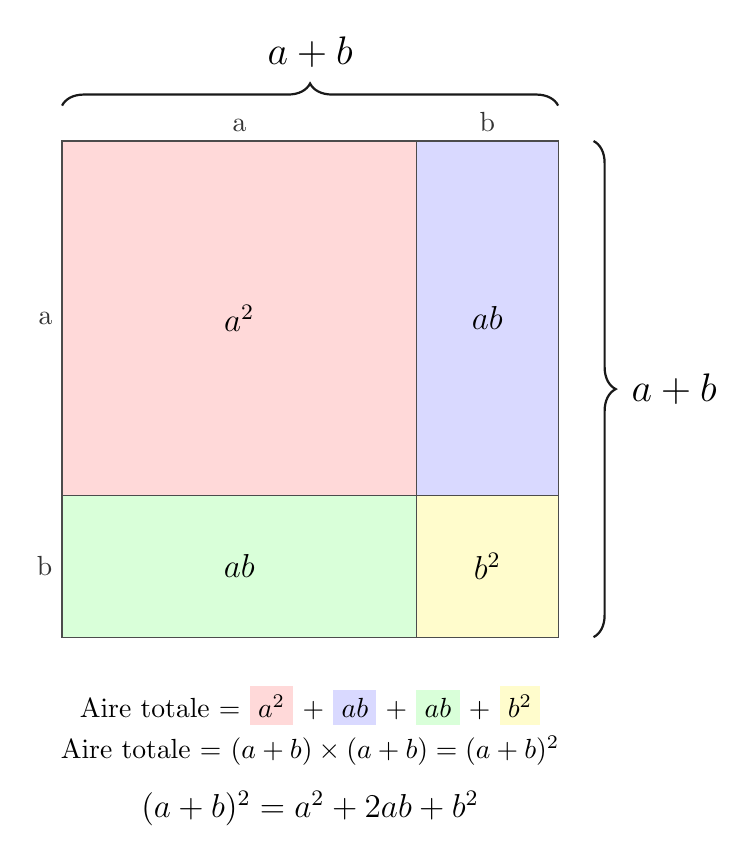
\begin{tikzpicture}[scale=1.5,font=\bfseries\large,quad/.style={draw=black!70,thin},label_side/.style={font=\normalfont\normalsize,color=black!80}]
			\def\la{3.0} \def\lb{1.2} \draw[quad, fill=red!15] (0,\lb) rectangle (\la, {\la+\lb}) node[pos=0.5] {$a^2$};
			\draw[quad, fill=blue!15] (\la,\lb) rectangle ({\la+\lb}, {\la+\lb}) node[pos=0.5] {$ab$};
			\draw[quad, fill=green!15] (0,0) rectangle (\la,\lb) node[pos=0.5] {$ab$};
			\draw[quad, fill=yellow!20] (\la,0) rectangle ({\la+\lb},\lb) node[pos=0.5] {$b^2$};
			\node[label_side, above] at ({\la/2}, {\la+\lb}) {a};
			\node[label_side, above] at ({\la+\lb/2}, {\la+\lb}) {b};
			\node[label_side, left] at (0, {\lb+\la/2}) {a};
			\node[label_side, left] at (0, {\lb/2}) {b};
			\draw[decorate, decoration={brace, amplitude=8pt}, thick, draw=black!90] (0, {\la+\lb+0.3}) -- ({\la+\lb}, {\la+\lb+0.3}) node[midway, above=10pt, font=\bfseries\Large, color=black] {$a + b$};
			\draw[decorate, decoration={brace, amplitude=8pt, mirror}, thick, draw=black!90] ({\la+\lb+0.3}, 0) -- ({\la+\lb+0.3}, {\la+\lb}) node[midway, right=10pt, font=\bfseries\Large, color=black] {$a + b$};
			\node[anchor=north, align=center, font=\normalfont\normalsize, yshift=-0.5cm] at ({(\la+\lb)/2}, 0) { Aire totale = \colorbox{red!15}{$a^2$} + \colorbox{blue!15}{$ab$} + \colorbox{green!15}{$ab$} + \colorbox{yellow!20}{$b^2$} \\[1mm] Aire totale = $(a + b) \times (a + b) = (a + b)^2$\\[3mm] \large $\Rarr (a + b)^2 = a^2 + 2ab + b^2$ };
		\end{tikzpicture}
	\end{center}
\end{rem}

	\newpage
\section{Exercices}
 {
  \small
  \setlength{\columnseprule}{0.6pt}
  \begin{multicols}{2}
	  \begin{exo}[Développement]
		  Développer et réduire les expressions suivantes:
		  \vspace*{-2mm}
		  \begin{multicols}{2}
			  \begin{enumerate}[label=\alph*)]
				  \item $3(x + 2) - 4(2 - 2x)$
				  \item $x(2x - 1) - 3(5 - x)$
				  \item $(3x + 1)x - 3(x - 2)$
				  \item $3(x - 5) - 2x(1 - 2x)$
			  \end{enumerate}
		  \end{multicols}
	  \end{exo}

	  \begin{exo}[Développement]
		  Développer et réduire les expressions suivantes:
		  \begin{enumerate}[label=\alph*)]
			  \item $(2x + 1)(3 - 2x)$
			  \item $(x - 3)(-x - 1)$
			  \item $(3x + 2)(5 - 2x)$
			  \item $(x - 1)(3x^{2} - 2)$
			  \item $(3 - x)(2x + 1) + 2(x + 2)$
			  \item $(x - 1)(2x - 1) - 3(3 + 2x)$
		  \end{enumerate}
	  \end{exo}

	  \begin{exo}[Factorisation]
		  Factoriser et réduire les expressions suivantes :
		  \vspace*{-2mm}
		  \begin{multicols}{2}
			  \begin{enumerate}[label=\alph*)]
				  \item $3x + 6$
				  \item $16x - 4$
				  \item $3x + 9$
				  \item $4x + 6$
				  \item $x^{2} + 3x$
				  \item $7x + 7x^{2}$
				  \item $8x^{2} + 6x$
				  \item $6x + 15x^{2}$
			  \end{enumerate}
		  \end{multicols}
	  \end{exo}

	  \begin{exo}[Factorisation]
		  Factoriser et réduire les expressions suivantes :
		  \begin{enumerate}[label=\alph*)]
			  \item $x(3x + 2) + x(5 - x)$
			  \item $4(5x + 2) + 2x(5x + 2)$
			  \item $(3x + 2)2x + 2x(2 - x)$
			  \item $(1 - 3x)(2 + x) + (1 - 3x)(5 - 2x)$
			  \item $(2x + 3)(4x + 3) - (2x + 3)(x - 1)$
			  \item $(x + 5)(4 - x) - (4 - x)$
			  \item $(x + 1)^{2} + (x + 1)(2x - 3)$
		  \end{enumerate}
	  \end{exo}

	  \begin{exo}[Association d'expressions algébriques]
		  Relier chaque expression de la première colonne avec sa forme développée dans la deuxième colonne.
		  \begin{tabular}{p{3.5cm} @{\hspace{10mm}} p{3cm}}
			  \vspace*{-2mm}
			  \begin{enumerate}[label=\arabic*)]
				  \item $(x + 7)^2$
				  \item $(x + \sqrt{7})^2$
				  \item $(x - 7)(x + 7)$
				  \item $(x^2 + 7)(x^2 - 7)$
				  \item $(x - 7)^2$
			  \end{enumerate}
			   &
			  \vspace*{-2mm}
			  \begin{enumerate}[label=\alph*)]
				  \item $x^2 - 14x + 49$
				  \item $x^2 + 49$
				  \item $x^2 + 14x + 49$
				  \item $x^2 + 7x + 49$
				  \item $x^2 + 2\sqrt{7}x + 7$
				  \item $x^4 - 49$
				  \item $x^2 - 49$
			  \end{enumerate}
			  \\
		  \end{tabular}
	  \end{exo}
	  \vfill~\columnbreak
	  \begin{exo}
		  À l'aide de l'identité remarquable donnée, développer les expressions algébriques suivantes.

		  \def\arraystretch{1.5}
		  \begin{tabular}{m{3.5cm}|m{3.5cm}}
			  $(a + b)^2 = a^2 + 2ab + b^2$ & $(a - b)^2 = a^2 - 2ab + b^2$ \\ \hline
			  \begin{enumerate}[label=\alph*)]
				  \item $(x + 3)^2$
				  \item $(2x + 8)^2$
				  \item $(4 + 3x)^2$
				  \item $\pa{\dfrac{1}{3} + y}^2$
			  \end{enumerate}
			                                &
			  \begin{enumerate}[label=\alph*)]
				  \item $(x - 9)^2$
				  \item $(3x - 4)^2$
				  \item $(2 - 5x)^2$
				  \item $(2y - \sqrt{3})^2$
			  \end{enumerate}
		  \end{tabular}
		  \begin{center}
			  \begin{tabular}{m{3.8cm}}
				  $(a + b)(a - b) = a^2 - b^2$ \\ \hline
				  \begin{enumerate}[label=\alph*)]
					  \item $(x + 14)(x - 14)$
					  \item $(7x + 9)(9 - 7x)$
					  \item $\left( \dfrac{2}{3} + \dfrac{x}{4} \right)\left( \dfrac{2}{3} - \dfrac{x}{4} \right)$
					  \item $\left( z + \dfrac{7}{4} \right)\left( z - \dfrac{35}{20} \right)$
				  \end{enumerate}
			  \end{tabular}
		  \end{center}
	  \end{exo}

	  \begin{exo}
		  À l'aide de l'identité remarquable donnée, factoriser les expressions algébriques suivantes.

		  \def\arraystretch{1.5}
		  \begin{tabular}{m{3.5cm}|m{3.5cm}}
			  $a^2 + 2ab + b^2 = (a + b)^2$ & $a^2 - 2ab + b^2 = (a - b)^2$ \\ \hline
			  \begin{enumerate}[label=\alph*)]
				  \item $x^2 + 10x + 25$
				  \item $9x^2 + 6x + 1$
				  \item $2y + 1 + y^2$
				  \item $4x^2 + 20x + 25$
			  \end{enumerate}
			                                &
			  \begin{enumerate}[label=\alph*)]
				  \item $x^2 - 8x + 16$
				  \item $9x^2 - 6x + 1$
				  \item $z^2 - z + \dfrac{1}{4}$
				  \item $25 + 25x^2 - 50x$
			  \end{enumerate}
		  \end{tabular}

		  \begin{center}
			  \begin{tabular}{m{3.8cm}}
				  $a^2 - b^2 = (a + b)(a - b)$ \\ \hline
				  \begin{enumerate}[label=\alph*)]
					  \item $a^2 - 144$
					  \item $9x^2 - 16$
					  \item $\dfrac{x^2}{4} - \dfrac{4}{9}$
					  \item $x^2 - 7$
				  \end{enumerate}
			  \end{tabular}
		  \end{center}
	  \end{exo}

	  \begin{exo}
		  À l'aide de l'identité remarquable la plus adaptée, développer les expressions algébriques suivantes.
		  \vspace*{-2mm}
		  \begin{multicols}{2}
			  \begin{enumerate}[label=\alph*)]
				  \item $(x + 11)^2$
				  \item $(3x - 7)^2$
				  \item $\left( x - \dfrac{2}{3} \right)\left( x + \dfrac{2}{3} \right)$
				  \item $(5x - 9)(5x + 9)$
				  \item $(2x - 1,5)^2$
				  \item $(x + \sqrt{2})^2$
			  \end{enumerate}
		  \end{multicols}
	  \end{exo}

	  \begin{exo}
		  À l'aide de l'identité remarquable la plus adaptée, factoriser, pour tout nombre réel $x$, les expressions algébriques suivantes.
		  \vspace*{-2mm}
		  \begin{multicols}{2}
			  \begin{enumerate}[label=\alph*)]
				  \item $x^2 + 14x + 49$
				  \item $9x^2 - 30x + 25$
				  \item $x^2 - \dfrac{16}{81}$
				  \item $16x^2 - 4900$
				  \item $6,25 + x^2 - 5x$
				  \item $x^2 + \sqrt{2}x + \dfrac{1}{2}$
			  \end{enumerate}
		  \end{multicols}
	  \end{exo}

	  \vfill~\columnbreak

	  \begin{exo}
		  Dans un plan, on considère une unité de longueur donnée. Soient les deux figures suivantes :

		  \begin{itemize}
			  \item Un rectangle dont les côtés mesurent $\pa{x - 1}$ et $\pa{x + 1}$
			  \item Un carré dont le côté mesure $x$ et dans lequel on a enlevé un carré de $1$ de côté.
		  \end{itemize}

		  \begin{center}
			  \begin{tikzpicture}[scale=0.7,>=Stealth]
				  \draw[very thick] (0,0) rectangle (4,2.5);
				  \draw[<->, thick] (-0.3,0) -- (-0.3,2.5) node[midway, above, sloped] {$x - 1$};
				  \draw[<->, thick] (0,-0.3) -- (4,-0.3) node[midway, below] {$x + 1$};
				  \begin{scope}[shift={(5.5,0)}]
					  \draw[very thick] (0,0) -- (4,0) -- (4,3.5) -- (1,3.5) -- (1,2.5) -- (0,2.5) -- cycle;
					  \draw[<->, thick] (0,2.7) -- (1,2.7) node[midway, above] {$1$};
					  \draw[<->, thick] (0,-0.3) -- (4,-0.3) node[midway, below] {$x$};
				  \end{scope}
			  \end{tikzpicture}
		  \end{center}

		  \begin{enumerate}
			  \item À quel plus grand intervalle $x$ peut-il appartenir ?
			  \item À l'aide d'une calculatrice, calculer l'aire de chacune de ces figures pour différentes valeurs de $x$.
			  \item Que peut-on conjecturer ?
			  \item Montrer que, pour tout $x > 1$, ces deux figures ont la même aire.
		  \end{enumerate}
	  \end{exo}

	  \begin{exo}
		  Dans cet exercice, on cherche à trouver une méthode pour calculer facilement $99^2$.

		  \begin{enumerate}
			  \item Compléter : \cmath{99^2 = (100 - \ldots)^2 = 100^2 - 2 \times \ldots \times \ldots + 1^2 = \ldots}
			  \item En remarquant que $999 = 1000 - 1$ et avec une méthode similaire, calculer $999^2$.
			  \item Avec une méthode similaire, calculer $1001^2$ et $95 \times 105$.
		  \end{enumerate}
	  \end{exo}

	  \begin{exo}
		  On considère l'expression littérale $A(x) = x^2 + 8x + 15$ définie pour tout réel $x$.
		  \begin{enumerate}
			  \item Montrer que $A(x) = (x + 4)^2 - 1$.
			  \item Montrer que $A(x) = (x + 3)(x + 5)$.
			  \item En choisissant la forme de $A(x)$ la plus adaptée à un calcul mental, calculer $A(0)$, $A(-3)$, $A(-4)$ et $A(-5)$.
		  \end{enumerate}
	  \end{exo}

	  \begin{exo}
		  On considère l'expression suivante définie pour tout $x$ : \cmath{B(x) = (4x + 5)^2 - (4x + 5)(7 - x)}

		  \begin{enumerate}
			  \item Pour tout $x$, développer et réduire $B(x)$.
			  \item Pour tout $x$, factoriser $B(x)$ à l'aide d'un facteur commun.
			  \item En déduire la résolution dans $\mathbb{R}$ de \cmath{20x^2 + 17x - 10 = 0}
		  \end{enumerate}
	  \end{exo}

	  \vfill~\columnbreak

	  \begin{exo}[Des cubes ...]
		  Cette figure montre la décomposition en plusieurs solides d'un cube d'arête $a + b$ où $a$ et $b$ sont des nombres réels positifs.

		  \begin{center}
			  \definecolor{cubevert}{RGB}{160,200,30}
			  \definecolor{cubeorange}{RGB}{250,185,40}
			  \definecolor{cubebleu}{RGB}{50,170,200}
			  \definecolor{cuberouge}{RGB}{225,85,35}
			  \newcommand{\boite}[7]{%
				  {\pgfmathsetmacro{\xb}{#1+#4}%
						  \pgfmathsetmacro{\yb}{#2+#5}%
						  \pgfmathsetmacro{\zb}{#3+#6}%
						  \filldraw[fill=#7!70!white, draw=white, line join=round, line width=0.4pt]
						  (#1,#2,\zb) -- (\xb,#2,\zb) -- (\xb,\yb,\zb) -- (#1,\yb,\zb) -- cycle;
						  \filldraw[fill=#7, draw=white, line join=round, line width=0.4pt]
						  (\xb,#2,#3) -- (\xb,\yb,#3) -- (\xb,\yb,\zb) -- (\xb,#2,\zb) -- cycle;
						  \filldraw[fill=#7!75!black, draw=white, line join=round, line width=0.4pt]
						  (#1,\yb,#3) -- (\xb,\yb,#3) -- (\xb,\yb,\zb) -- (#1,\yb,\zb) -- cycle;}%
			  }

			  \begin{tikzpicture}[scale=1.1, x={(-0.21cm,-0.12cm)}, y={(0.21cm,-0.12cm)}, z={(0cm,0.24cm)}, font=\small]
				  \begin{scope}
					  \boite{0}{0}{0}{2}{2}{2}{cubevert}
					  \node[right=-1mm] at (0,2,1) {$a$};
				  \end{scope}
				  \begin{scope}[xshift=1.9cm]
					  \boite{0}{0}{0}{2}{2}{2}{cubevert}
					  \boite{2}{0}{0}{1}{2}{2}{cubeorange}
					  \boite{0}{0}{2}{2}{2}{1}{cubeorange}
					  \node[right=-3mm] at (0,3,3.2) {$b$};
					  \node[right=-3mm] at (0,3,1.6) {$a$};
				  \end{scope}
				  \begin{scope}[xshift=3.8cm]
					  \boite{2}{0}{0}{1}{2}{2}{cubeorange}
					  \boite{0}{2}{0}{2}{1}{2}{cubeorange}
					  \boite{0}{0}{2}{2}{2}{1}{cubeorange}
					  \node[right=-3mm] at (0,3,3.2) {$b$};
					  \node[right=1mm] at (0,2.3,0.6) {$a$};
				  \end{scope}
				  \begin{scope}[xshift=0.8cm, yshift=-1.5cm]
					  \boite{2}{0}{0}{1}{2}{2}{cubeorange}
					  \boite{0}{2}{0}{2}{1}{2}{cubeorange}
					  \boite{0}{0}{2}{2}{2}{1}{cubeorange}
					  \boite{2}{2}{0}{1}{1}{2}{cubebleu}
					  \boite{2}{0}{2}{1}{2}{1}{cubebleu}
					  \boite{0}{2}{2}{2}{1}{1}{cubebleu}
					  \node[right=-1mm] at (0,3,2.5) {$b$};
					  \node[right=-1mm] at (0,3,1)   {$a$};
				  \end{scope}
				  \begin{scope}[xshift=2.7cm,yshift=-1.5cm]
					  \boite{2}{0}{0}{1}{2}{2}{cubeorange}
					  \boite{0}{2}{0}{2}{1}{2}{cubeorange}
					  \boite{0}{0}{2}{2}{2}{1}{cubeorange}
					  \boite{2}{2}{0}{1}{1}{2}{cubebleu}
					  \boite{2}{0}{2}{1}{2}{1}{cubebleu}
					  \boite{0}{2}{2}{2}{1}{1}{cubebleu}
					  \boite{2}{2}{2}{1}{1}{1}{cuberouge}
					  \node[right=-1mm] at (0,3,2.5) {$b$};
					  \node[right=-1mm] at (0,3,1)   {$a$};
				  \end{scope}
			  \end{tikzpicture}
		  \end{center}

		  \begin{enumerate}
			  \item Pour chaque couleur de solide (vert, jaune, bleu et rouge) :
			        \begin{enumerate}
				        \item Déterminer le nombre de solides.
				        \item Déterminer le volume d'un solide en fonction de $a$ et $b$.
			        \end{enumerate}
			  \item Montrer que $(a + b)^3 = a^3 + 3a^2b + 3ab^2 + b^3$.
			  \item Cette égalité est-elle démontrée pour tous $a$ et $b$ ?
		  \end{enumerate}
	  \end{exo}

	  \begin{exo}[... et des carrés]
		  On considère le carré $ABCD$ de côtés $6\text{ cm}$ et quatre points $M$, $N$, $P$, $Q$ tels que $AM = BN = CP = DQ$

		  On admet que $MNPQ$ est un carré et on note $x = BM$

		  \begin{center}
			  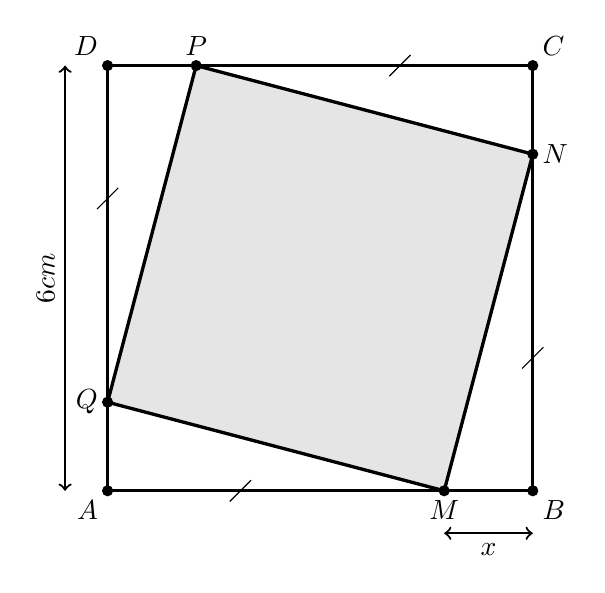
\begin{tikzpicture}[scale=0.9]
				  \coordinate (A) at (0,0);
				  \coordinate (B) at (6,0);
				  \coordinate (C) at (6,6);
				  \coordinate (D) at (0,6);
				  \draw[very thick] (A) -- (B) -- (C) -- (D) -- cycle;
				  \node[below left] at (A) {$A$};
				  \node[below right] at (B) {$B$};
				  \node[above right] at (C) {$C$};
				  \node[above left] at (D) {$D$};
				  \coordinate (M) at (4.75,0);
				  \coordinate (N) at (6,4.75);
				  \coordinate (P) at (1.25,6);
				  \coordinate (Q) at (0,1.25);
				  \draw[very thick, fill=black!10] (M) -- (N) -- (P) -- (Q) -- cycle;
				  \node[below] at (M) {$M$};
				  \node[right] at (N) {$N$};
				  \node[above] at (P) {$P$};
				  \node[left] at (Q) {$Q$};
				  \draw[<->, thick] (-0.6,0) -- (-0.6,6) node[midway, above, sloped] {$6\text{ cm}$};
				  \draw[<->, thick] (4.75,-0.6) -- (6,-0.6) node[midway, below] {$x$};
				  \draw[shift={(1.875,0)}] (-0.15,-0.15) -- (0.15,0.15);
				  \draw[shift={(6,1.875)}] (-0.15,-0.15) -- (0.15,0.15);
				  \draw[shift={(4.125,6)}] (-0.15,-0.15) -- (0.15,0.15);
				  \draw[shift={(0,4.125)}] (-0.15,-0.15) -- (0.15,0.15);
				  \foreach \pt in {A,B,C,D,M,N,P,Q} { \filldraw[black] (\pt) circle (2pt); }
			  \end{tikzpicture}
		  \end{center}

		  \begin{enumerate}
			  \item Justifier que l'aire $\mathcal{A}$ du carré $MNPQ$ a pour valeur : \cmath{\mathcal{A} = 2x^2 - 12x + 36}
		  \end{enumerate}

		  \textbf{Aide :} $\text{Aire}(MNPQ) = \text{Aire}(ABCD) - 4 \times \text{Aire}(AMQ)$

		  \begin{enumerate}[resume]
			  \item \begin{enumerate}
				        \item Montrer que : \cmath{2(x - 2)(x - 4)\ =\ 2x^2 - 12x + 16}
				        \item Déterminer la ou les valeurs de $x$ afin que l'aire du carré $MNPQ$ soit égale aux $\dfrac{5}{9}$ de celle du carré $ABCD$.
			        \end{enumerate}
		  \end{enumerate}
	  \end{exo}

	  \vfill~
  \end{multicols}
 }

	\chapter{Multiples et diviseurs}

\section{Multiples et diviseurs}

\begin{definition}[Multiple et diviseur]
	Soit $a$ et $b$ deux entiers naturels.

	On dit que $a$ est un \textbf{multiple} de $b$ s'il existe un entier $k$ tel que :
	\[
		a = k \times b
	\]

	On dit alors que $b$ est un \textbf{diviseur} de $a$.
\end{definition}

\begin{exemple}
	$15$ est un multiple de $3$, car $15 = 5 \times 3$ (avec $k = 5$).
\end{exemple}

\begin{methode}[Démontrer qu'un nombre est multiple ou diviseur]
	Les affirmations suivantes sont-elles vraies ou fausses ?
	\begin{multicols}{2}
		\begin{enumerate}[label=\alph*)]
			\item $36$ est un multiple de $12$.
			\item $28$ est un multiple de $8$.
			\item $6$ est un diviseur de $54$.
			\item $7$ est un diviseur de $24$.
		\end{enumerate}
	\end{multicols}

	\begin{correction}
		\nline
		\begin{enumerate}[label=\alph*)]
			\item \textbf{VRAI :} $36$ est un multiple de $12$, car $36 = 3 \times 12$ avec $k = 3$.
			\item \textbf{FAUX :} $28$ n'est pas un multiple de $8$ car il n'existe aucun entier $k$ tel que $28 = k \times 8$.
			\item \textbf{VRAI :} $6$ est un diviseur de $54$, car $54 = 9 \times 6$ avec $k = 9$.
			\item \textbf{FAUX :} $7$ n'est pas un diviseur de $24$ car il n'existe aucun entier $k$ tel que $24 = k \times 7$.
		\end{enumerate}
	\end{correction}
\end{methode}

\begin{propriete}[Somme de multiples]
	La \textbf{somme} de deux multiples d'un entier naturel $a$ est un multiple de $m$.

	Autrement dit, si $b = k_1 \times m$ et $c = k_2 \times m$ (avec $k_1$ et $k_2$ entiers), alors :
	\[
		b + c = k \times m\qquad \text{avec}\; k\; {entier}
	\]
\end{propriete}

\begin{exemple}
	$700$ et $21$ sont des multiples de $7$, donc $721 = 700 + 21$ est aussi un multiple de $7$.
\end{exemple}

\begin{demo}[La somme de deux multiples de $m$ est un multiple de $m$]
	Soit $m$ un entier naturel. Soit $b$ et $c$ deux multiples de $m$.

	Comme $b$ est un multiple de $m$, il existe un entier $k_1$ tel que $b = m \times k_1$.

	Comme $c$ est un multiple de $m$, il existe un entier $k_2$ tel que $c = m \times k_2$.

	Alors :
	\[
		b + c = m \times k_1 + m \times k_2 = m \times (k_1 + k_2) = m \times k, \quad \text{où } k = k_1 + k_2.
	\]

	$k = k_1 + k_2$ est un entier, donc $b + c$ est de la forme $m \times k$ avec $k$ entier.

	Ainsi, $b + c$ est bien un multiple de $m$.
\end{demo}

\newpage

\begin{methode}[Résoudre un problème avec des multiples]
	Montrer que la somme de trois entiers consécutifs est toujours un multiple de $3$.

	\begin{correction}
		Soit trois entiers consécutifs notés $n$, $n + 1$ et $n + 2$, où $n$ est un entier naturel quelconque.

		Leur somme $S$ vaut :
		\[
			S = n + (n + 1) + (n + 2) = 3n + 3 = 3(n + 1).
		\]

		En posant $k = n + 1$ ($k$ est un entier), on a $S = 3k$.

		$S$ est donc bien un multiple de $3$.
	\end{correction}
\end{methode}

\section{Nombres pairs et impairs}

\begin{definition}[Parité]
	Un nombre entier est \textbf{pair} s'il est un multiple de $2$.

	Un nombre entier est \textbf{impair} s'il n'est pas pair.

	\begin{itemize}
		\item Un nombre pair s'écrit sous la forme $2k$, avec $k$ entier.
		\item Un nombre impair s'écrit sous la forme $2k + 1$, avec $k$ entier.
	\end{itemize}
\end{definition}

\begin{exemple}
	\nline
	\begin{itemize}
		\item $34$ est pair car $34 = 2 \times 17$.
		\item $57$ est impair car $57 = 2 \times 28 + 1$.
	\end{itemize}
\end{exemple}

\begin{propriete}[Règles de parité]
	\nline
	\begin{center}
		\def\arraystretch{1.4}%
		\begin{tabular}{c|c|c}%
			$+$ ou $-$ & pair   & impair \\
			\hline
			pair       & pair   & impair \\
			impair     & impair & pair   \\
		\end{tabular}
		\qquad\qquad
		\begin{tabular}{c|c|c}%
			$\times$ & pair & impair \\
			\hline
			pair     & pair & pair   \\
			impair   & pair & impair \\
		\end{tabular}
	\end{center}
\end{propriete}

\begin{demo}
	\nline
	\begin{enumerate}
		\item \textbf{Produit d'un pair et d'un impair :}

		      Soit $n$ un nombre pair et $m$ un nombre impair.

		      Il existe deux entiers $k$ et $p$ tels que $n = 2k$ et $m = 2p + 1$.

		      On calcule leur produit :
		      \[
			      n \times m = 2k \times (2p + 1) = 2 \times [k(2p + 1)]
		      \]
		      En posant $K = k(2p + 1)$, qui est un entier, on obtient $n \times m = 2K$.

		      Le produit est donc de la forme $2K$ : c'est un nombre \textbf{pair}.

		\item \textbf{Produit de deux impairs :}

		      Soit $n$ et $m$ deux nombres impairs.

		      Il existe deux entiers $k$ et $p$ tels que $n = 2k + 1$ et $m = 2p + 1$.

		      On développe leur produit :
		      \begin{align*}
			      n \times m & = (2k + 1)(2p + 1)   \\
			                 & = 4kp + 2k + 2p + 1  \\
			                 & = 2(2kp + k + p) + 1
		      \end{align*}
		      En posant $K' = 2kp + k + p$, qui est un entier, on obtient $n \times m = 2K' + 1$.

		      Le produit est donc de la forme $2K' + 1$ : c'est un nombre \textbf{impair}.
	\end{enumerate}
\end{demo}

\begin{methode}[Déterminer la parité d'un nombre]
	Quelle est la parité de $\np{5678984}^2 + 1$ ?

	\begin{correction}
		$\def\arraystretch{1.2}%
			\begin{array}{rl}%
				\np{5678984}^2 = & \np{5678984} \times \np{5678984}                 \\
				=                & \text{PAIR} \times \text{PAIR} \Rarr \text{PAIR} \\
				=                & 2k, \text{ avec } k \text{ entier.}
			\end{array}$%

		\ms

		Donc $5\,678\,984^2 + 1 = 2k + 1$, ce qui prouve que ce nombre est \textbf{impair}.
	\end{correction}
\end{methode}

\begin{propriete}[Carré d'un impair]
	Le carré d'un nombre impair est un nombre impair.
\end{propriete}

\begin{demo}[Le carré d'un impair est impair]
	Soit $a$ un nombre impair.

	Il s'écrit $a = 2k + 1$, avec $k$ entier.

	Alors :
	\[
		a^2 = \pa{2k + 1}^2 = 4k^2 + 4k + 1 = 2\pa{2k^2 + 2k} + 1 = 2k' + 1,
	\]

	\ldots avec $k' = 2k^2 + 2k$ entier (somme de produits d'entiers).

	Comme $a^2$ s'écrit sous la forme $2k' + 1$, $a^2$ est bien impair.
\end{demo}

\begin{methode}[Résoudre un problème de parité]
	Montrer que le produit de deux entiers consécutifs est toujours un nombre pair.

	\begin{correction}
		Soit deux entiers consécutifs $n$ et $n + 1$.
		\begin{itemize}
			\item \textbf{Cas 1 :} $n$ est pair.

			      Alors $n = 2k$ avec $k$ entier, et :

			      \[
				      n(n + 1) = 2k(2k + 1) = 2k_1, \quad \text{avec } k_1 = k(2k + 1) \text{ entier}.
			      \]

			      Donc $n(n + 1)$ est pair.

			\item \textbf{Cas 2 :} $n$ est impair.

			      Alors $n = 2k + 1$ avec $k$ entier, et :

			      \[
				      n(n + 1) = (2k + 1)(2k + 2) = 2(2k + 1)(k + 1) = 2k_2, \quad \text{avec } k_2 = (2k + 1)(k + 1) \text{ entier}.
			      \]

			      Donc $n(n + 1)$ est pair.
		\end{itemize}

		\textbf{Conclusion :} Dans tous les cas, le produit de deux entiers consécutifs est un nombre pair.
	\end{correction}
\end{methode}

\section{Nombres premiers}

\begin{definition}[Nombre premier]
	Un entier naturel est \textbf{premier} s'il possède exactement deux diviseurs distincts : $1$ et lui-même.
\end{definition}

\begin{exemple}[Nombres premiers]
	Les premiers nombres premiers sont : $2, 3, 5, 7, 11, 13, 17, 19, 23, \ldots$ (il y en a une infinité).

\end{exemple}

\begin{rem}
	Le nombre $1$ n'est \textbf{pas} premier car il n'a qu'un seul diviseur ($1$).
\end{rem}

\newpage

\begin{propriete}[Critère d'arrêt]
	Soit $n$ un entier naturel supérieur ou égal à $2$.

	Si $n$ n'est pas un nombre premier, alors il possède au moins un diviseur premier $p$ tel que :
	\[
		p \leqslant \sqrt{n}
	\]
\end{propriete}

\begin{demo}
	Soit $n \geqslant 2$ un entier non premier (on dit aussi composé).

	$n$ admet donc au moins deux diviseurs stricts distincts de $1$ et de lui-même.

	On peut donc écrire $n = a \times b$, où $a$ et $b$ sont deux entiers naturels vérifiant $1 < a \leqslant b < n$.

	Raisonnons par l'absurde et supposons que $a > \sqrt{n}$ et $b > \sqrt{n}$.

	En multipliant ces deux inégalités strictement positives membre à membre, on obtient :
	\[
		a \times b > \sqrt{n} \times \sqrt{n}\iff n > n
	\]

	Ce qui est absurde.

	L'hypothèse de départ est donc fausse : l'un au moins des deux facteurs est inférieur ou égal à $\sqrt{n}$.
\end{demo}
\begin{methode}[Vérifier si un nombre est premier]
	Démontrer que le nombre $97$ est premier.

	\begin{correction}
		On calcule $\sqrt{97} \approx 9{,}8$. On teste la divisibilité de $97$ par tous les \textbf{nombres premiers} inférieurs ou égaux à $\sqrt{97}$, c'est-à-dire : $2$, $3$, $5$ et $7$.

		\begin{itemize}
			\item \textbf{2 :} Non - $97$ est impair (il se termine par $7$).
			\item \textbf{3 :} Non - La somme de ses chiffres vaut $9 + 7 = 16$, qui n'est pas un multiple de $3$.
			\item \textbf{5 :} Non - $97$ ne se termine ni par $0$ ni par $5$.
			\item \textbf{7 :} Non - $97 = 7 \times 13 + 6$ (la division euclidienne donne un reste non nul).
		\end{itemize}

		Comme $97$ n'est divisible par aucun nombre premier inférieur ou égal à $\sqrt{97}$, le nombre $97$ est un \textbf{nombre premier}.
	\end{correction}
\end{methode}

\begin{propriete}[Décomposition en facteurs premiers]
	Tout entier $n \geqslant 2$ se décompose de manière unique (à l'ordre des facteurs près) sous la forme :
	\[
		n = p_1^{a_1} \times p_2^{a_2} \times \cdots \times p_k^{a_k}
	\]

	\ldots où $p_1, p_2, \ldots, p_k$ sont des nombres premiers distincts et $a_1, a_2, \ldots, a_k$ sont des entiers naturels non nuls.
\end{propriete}

\begin{exemple}[Décomposition]
	\[
		\def\arraystretch{1.2}%
		\begin{array}{r|l}%
			300 & 2 \\
			150 & 2 \\
			75  & 3 \\
			25  & 5 \\
			5   & 5 \\
			1   &
		\end{array}\qquad\Rarr\qquad 300 = 2 \times 2 \times 3 \times 5 \times 5 = 2^2 \times 3 \times 5^2
	\]
\end{exemple}

\newpage

\begin{definition}[Fraction irréductible]
	Une fraction est dite \textbf{irréductible} lorsque son numérateur et son dénominateur n'ont aucun diviseur commun autre que $1$.
\end{definition}

\begin{methode}[Rendre une fraction irréductible]
	Rendre irréductible la fraction $\dfrac{60}{126}$.

	\begin{correction}
		On décompose le numérateur et le dénominateur en produit de facteurs premiers :
		\[
			\def\arraystretch{1.2}%
			\begin{array}{r|l}%
				60 & 2 \\
				30 & 2 \\
				15 & 3 \\
				5  & 5 \\
				1  &
			\end{array}%
			\quad \Rarr \quad 60 = 2 \times 2 \times 3 \times 5 \qquad\qquad \def\arraystretch{1.2}%
			\begin{array}{r|l}%
				126 & 2 \\
				63  & 3 \\
				21  & 3 \\
				7   & 7 \\
				1   &
			\end{array}%
			\quad \Rarr \quad 126 = 2 \times 3 \times 3 \times 7
		\]

		\ms

		On simplifie les facteurs communs ($2$ et $3$) :
		\[
			\frac{60}{126} = \frac{\cancel{2} \times 2 \times \cancel{3} \times 5}{\cancel{2} \times \cancel{3} \times 3 \times 7} = \frac{2 \times 5}{3 \times 7} = \frac{10}{21}
		\]

		$10$ et $21$ n'ont aucun diviseur commun autre que $1$, donc $\dfrac{10}{21}$ est la forme irréductible.
	\end{correction}
\end{methode}

\begin{rem}[Crible d'Ératosthène]
	Le crible d'Ératosthène est un procédé algorithmique permettant de trouver tous les nombres premiers inférieurs ou égaux à une valeur donnée $N$ (ici $N = 100$).

	% \begin{enumerate}
	% 	\item \textbf{Initialisation :} Écrire tous les nombres entiers de $2$ à $100$ dans un tableau.
	% 	\item \textbf{Élimination du premier multiple :} Le premier nombre non barré est $2$. Il est \textbf{premier}. On barre ensuite tous ses multiples strictement supérieurs à $2$ ($4, 6, 8, \dots, 100$).
	% 	\item \textbf{Réitération :} Le nombre suivant non barré est $3$. Il est \textbf{premier}. On barre tous ses multiples strictement supérieurs à $3$ qui ne le sont pas encore ($9, 15, 21, \dots$).
	% 	\item \textbf{Condition d'arrêt :} On répète l'opération avec le premier nombre non barré suivant ($5$, puis $7$).
	%
	% 	      Comme $\sqrt{100} = 10$, il suffit de tester les multiples des nombres premiers inférieurs ou égaux à $10$ (c'est-à-dire $2$, $3$, $5$ et $7$).
	% 	\item \textbf{Conclusion :} Tous les nombres restant non barrés dans le tableau sont les \textbf{nombres premiers} inférieurs ou égaux à $100$.
	% \end{enumerate}

	\begin{center}
		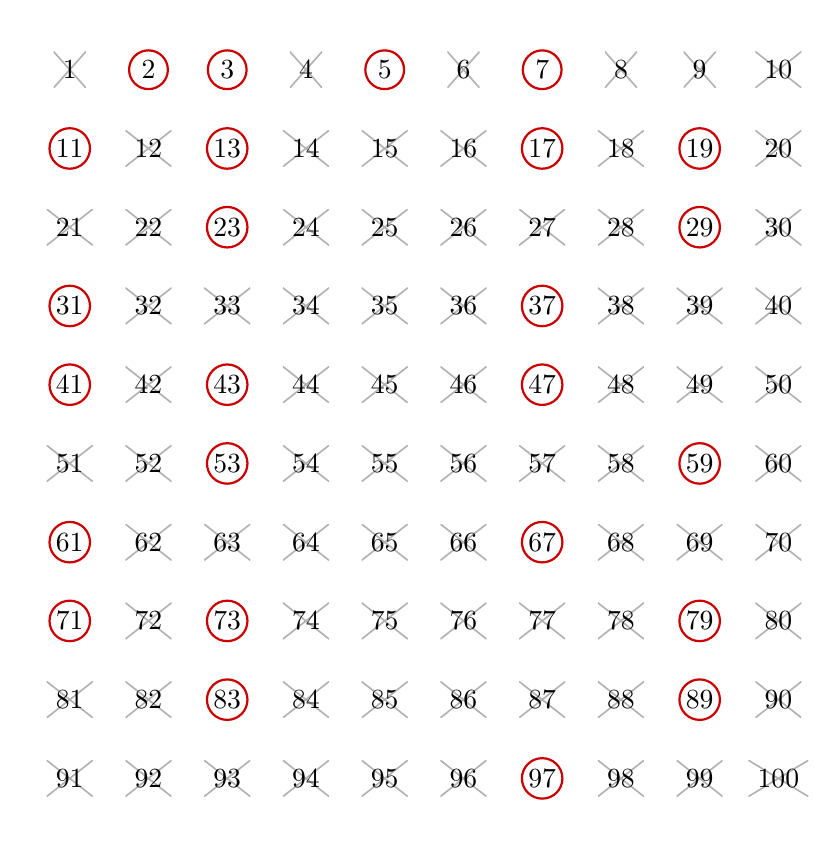
\begin{tikzpicture}[prime/.style={draw=red!80!black, thick, circle, fill=white, inner sep=1pt, minimum size=14pt},crossed/.style={ path picture={ \draw[gray!60, line width=0.6pt] (path picture bounding box.south west) -- (path picture bounding box.north east) (path picture bounding box.south east) -- (path picture bounding box.north west); } } ]
			\foreach \n in {1,...,100} { \pgfmathtruncatemacro{\r}{int((\n-1)/10)} \pgfmathtruncatemacro{\c}{\n - \r*10} \node[crossed] at (\c, 10-\r) {\n}; }
			\foreach \p in {2,3,5,7,11,13,17,19,23,29,31,37,41,43,47,53,59,61,67,71,73,79,83,89,97} { \pgfmathtruncatemacro{\r}{int((\p-1)/10)} \pgfmathtruncatemacro{\c}{\p - \r*10} \filldraw[white] (\c, 10-\r) circle (15pt); \node[prime] at (\c, 10-\r) {\p}; }
		\end{tikzpicture}
	\end{center}
\end{rem}

	\chapter{Ensembles de nombres et intervalles}

\section{Ensembles de nombres}

\subsection{L'ensemble des entiers naturels $\N$}

\begin{df}
	\nline
	\begin{wrapstuff}[r,width=3cm]
		\begin{center}
			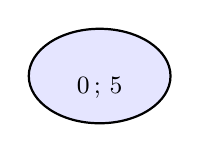
\begin{tikzpicture}[scale=0.75]
				\draw[thick, fill=blue!10] (0,0) ellipse (1.2cm and 0.8cm);
				\node at (0,0.3) {\textbf{$\N$}};
				\node[font=\small] at (0,-0.2) {$0 \,;\, 5$};
			\end{tikzpicture}
		\end{center}
	\end{wrapstuff}

	L'\textbf{ensemble des entiers naturels}, noté $\N$, est l'ensemble des entiers positifs ou nuls.
	\[
		\N = \{0\,;\, 1\,;\, 2\,;\, 3\,;\, 4\,;\, \dots\}
	\]
\end{df}

\begin{ex}
	$5 \in \N$ \quad et \quad $0 \in \N$.
\end{ex}

\subsection{L'ensemble des entiers relatifs $\Z$}

\begin{df}
	\nline
	\begin{wrapstuff}[r,width=4cm]
		\begin{center}
			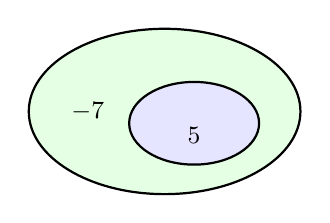
\begin{tikzpicture}[scale=0.75]
				\draw[thick, fill=green!10] (0,0) ellipse (2.3cm and 1.4cm);
				\node at (0,1) {\textbf{$\Z$}};
				\node[font=\small] at (-1.3,0) {$-7$};
				\draw[thick, fill=blue!10] (0.5,-0.2) ellipse (1.1cm and 0.7cm);
				\node at (0.5,0.05) {\textbf{$\N$}};
				\node[font=\small] at (0.5,-0.4) {$5$};
			\end{tikzpicture}
			\vspace*{-10mm}
		\end{center}
	\end{wrapstuff}
	L'\textbf{ensemble des entiers relatifs}, noté $\Z$, est l'ensemble des entiers positifs, négatifs ou nuls.
	\[
		\Z = \{\dots\,;\, - 3\,;\, - 2\,;\, - 1\,;\, 0\,;\, 1\,;\, 2\,;\, 3\,;\, \dots\}
	\]
\end{df}

\begin{ex}
	$-7 \in \Z$ \quad et \quad $5 \in \Z$ (tout entier naturel est aussi un entier relatif).
\end{ex}

\subsection{L'ensemble des nombres décimaux $\D$}

\begin{df}
	\nline
	\begin{wrapstuff}[r,width=5cm]
		\begin{center}
			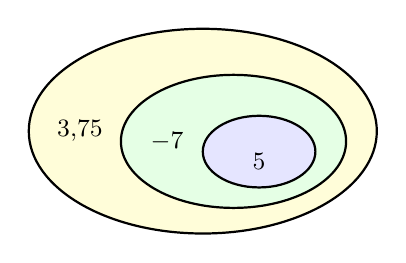
\begin{tikzpicture}[scale=0.65]
				\draw[thick, fill=yellow!15] (0,0) ellipse (3.4cm and 2cm);
				\node at (0,1.5) {\textbf{$\D$}};
				\node[font=\small] at (-2.4,0) {$3{,}75$};
				\draw[thick, fill=green!10] (0.6,-0.2) ellipse (2.2cm and 1.3cm);
				\node at (0.6,0.7) {\textbf{$\Z$}};
				\node[font=\small] at (-0.7,-0.2) {$-7$};
				\draw[thick, fill=blue!10] (1.1,-0.4) ellipse (1.1cm and 0.7cm);
				\node at (1.1,-0.15) {\textbf{$\N$}};
				\node[font=\small] at (1.1,-0.6) {$5$};
			\end{tikzpicture}
			\vspace*{-20mm}
		\end{center}
	\end{wrapstuff}

	L'\textbf{ensemble des nombres décimaux}, noté $\D$, est l'ensemble des nombres qui peuvent s'écrire sous la forme $\frac{a}{10^n}$, où $a \in \Z$ et $n \in \N$.

\end{df}

\begin{remarque}
	Un nombre décimal possède un \textbf{nombre fini de chiffres après la virgule}.
\end{remarque}

\begin{ex}
	$3{,}75 \in \D$ \quad car \quad $3{,}75 = \dfrac{375}{10^2}$
\end{ex}

\subsection{L'ensemble des nombres rationnels $\Q$}

\begin{df}
	\nline
	\begin{wrapstuff}[r,width=5.7cm]
		\begin{center}
			\begin{tikzpicture}[scale=0.55]
				\draw[thick, fill=orange!15] (0,0) ellipse (4.5cm and 2.6cm);
				\node at (0,2.1) {\textbf{$\Q$}};
				\node[font=\small] at (-3.2,0) {$\dfrac{1}{3}$};
				\draw[thick, fill=yellow!15] (0.7,-0.2) ellipse (3.3cm and 1.9cm);
				\node at (0.7,1.3) {\textbf{$\D$}};
				\node[font=\small] at (-1.7,-0.2) {$3{,}75$};
				\draw[thick, fill=green!10] (1.3,-0.4) ellipse (2.2cm and 1.2cm);
				\node at (1.3,0.4) {\textbf{$\Z$}};
				\node[font=\small] at (0,-0.4) {$-7$};
				\draw[thick, fill=blue!10] (1.8,-0.6) ellipse (1cm and 0.6cm);
				\node at (1.8,-0.35) {\textbf{$\N$}};
				\node[font=\small] at (1.8,-0.87) {$5$};
			\end{tikzpicture}
		\end{center}
		\vspace*{-10mm}
	\end{wrapstuff}

	L'\textbf{ensemble des nombres rationnels}, noté $\Q$, est l'ensemble des nombres qui peuvent s'écrire sous la forme d'une fraction $\frac{a}{b}$, avec $a \in \Z$ et $b \in \Z^*$ ($b \neq 0$).

	Son écriture décimale possède une \textbf{suite de chiffres qui se répète périodiquement} après la virgule.
\end{df}

\begin{ex}
	$\dfrac{1}{3} \in \Q$ \quad car \quad $\dfrac{1}{3} = 0{,}3333\dots$ (non décimal, mais rationnel ... voir démonstration ci-dessous).
\end{ex}

\begin{demo}[$\frac{1}{3}$ n'est pas un nombre décimal]
	On effectue un raisonnement par l'absurde.

	Supposons que $\tfrac{1}{3}$ soit un nombre décimal.

	Alors, par définition, il pourrait s'écrire sous la forme :

	\[
		\frac{1}{3} = \frac{a}{10^n} \quad \text{avec } a \in \Z \text{ et } n \in \N
	\]

	En effectuant le produit en croix, on obtient :

	\[
		3 \times a = 10^n \times 1 \implies 3a = 10^n
	\]

	Cela signifie que $10^n$ doit être un multiple de $3$.

	Or, un nombre est divisible par $3$ si la somme de ses chiffres est un multiple de $3$.

	La somme des chiffres de $10^n$ (qui s'écrit $1$ suivi de $n$ zéro(s)) est égale à $1 + 0 + \dots + 0 = 1$.

	Puisque $1$ n'est pas divisible par $3$, $10^n$ n'est jamais un multiple de $3$.

	Nous obtenons une \textbf{contradiction}.

	L'hypothèse de départ est donc fausse : $\frac{1}{3}$ n'est pas un nombre décimal $\pa{\frac{1}{3} \notin \D}$.
\end{demo}

\subsection{L'ensemble des nombres réels $\R$}

\begin{df}
	L'\textbf{ensemble des nombres réels}, noté $\R$, est l'ensemble de tous les nombres connus en Seconde (représentés par tous les points de la droite graduée).

	Il contient les nombres rationnels ainsi que les \textbf{nombres irrationnels}, qui ne peuvent pas s'écrire sous forme de fraction.
\end{df}

\begin{ex}
	$\sqrt{2} \in \R$ \quad et \quad $\pi \in \R$ \quad (ce sont des nombres irrationnels).
\end{ex}

\begin{demo}[$\sqrt{2}$ n'est pas un nombre rationnel]

	On effectue à nouveau un raisonnement par l'absurde.

	Supposons que $\sqrt{2}$ soit un nombre rationnel.

	Alors $\sqrt{2}$ s'écrit sous la forme d'une fraction irréductible :

	\[
		\sqrt{2} = \frac{a}{b} \quad \text{avec } a \in \N^*, b \in \N^*
	\]

	En élevant au carré des deux côtés :

	\[
		2 = \frac{a^2}{b^2} \implies a^2 = 2b^2
	\]

	Comme $a^2$ s'écrit sous la forme $2k$ (avec $k = b^2$), $a^2$ est un nombre \textbf{pair}.

	Or, le carré d'un nombre impair est impair. Ainsi, comme $a^2$ est pair, \textbf{$a$ est nécessairement pair}.

	Puisque $a$ est pair, il existe un entier $k \in \N^*$ tel que $a = 2k$.

	En remplaçant dans l'égalité $a^2 = 2b^2$ :

	\[
		(2k)^2 = 2b^2 \implies 4k^2 = 2b^2 \implies b^2 = 2k^2
	\]

	De même, $b^2$ s'écrit $2k^2$, donc $b^2$ est pair, ce qui implique que \textbf{$b$ est aussi pair}.

	Si $a$ et $b$ sont tous les deux pairs, ils sont tous les deux divisibles par $2$.

	Cela contredit le fait que $\dfrac{a}{b}$ est irréductible.

	Nous obtenons une \textbf{contradiction}.

	L'hypothèse de départ est donc fausse : $\sqrt{2}$ n'est pas un nombre rationnel ($\sqrt{2} \notin \Q$).
\end{demo}

\begin{prop}[Inclusion globale des ensembles de nombres]

	\[
		\N \subset \Z \subset \D \subset \Q \subset \R
	\]

\end{prop}

\begin{center}
	\begin{tikzpicture}[scale=0.85]
		\draw[thick, fill=red!10] (0,0) ellipse (5.8cm and 3.2cm);
		\node at (0,2.7) {\Large \textbf{$\R$}};
		\node[font=\small] at (-4.5,0.5) {$\pi$};
		\node[font=\small] at (-4.2,-0.8) {$\sqrt{2}$};
		\draw[thick, fill=orange!15] (0.8,-0.2) ellipse (4.5cm and 2.5cm);
		\node at (0.8,1.9) {\Large \textbf{$\Q$}};
		\node[font=\small] at (-2.5,0) {$\dfrac{1}{3}$};
		\draw[thick, fill=yellow!15] (1.5,-0.4) ellipse (3.4cm and 1.8cm);
		\node at (1.5,1.1) {\Large \textbf{$\D$}};
		\node[font=\small] at (-0.8,-0.4) {$3{,}75$};
		\draw[thick, fill=green!10] (2.1,-0.6) ellipse (2.3cm and 1.2cm);
		\node at (2.1,0.2) {\Large \textbf{$\Z$}};
		\node[font=\small] at (0.7,-0.6) {$-7$};
		\draw[thick, fill=blue!10] (2.7,-0.8) ellipse (1.2cm and 0.6cm);
		\node at (2.7,-0.55) {\Large \textbf{$\N$}};
		\node[font=\small] at (2.7,-1.05) {$5$};
	\end{tikzpicture}
\end{center}

\begin{ex}
	\nline
	\begin{enumerate}
		\item \textbf{Étude de $A = \dfrac{7}{6} - \dfrac{5}{4} + \dfrac{1}{12}$ :}

		      On met tout au même dénominateur :

		      \[
			      A = \frac{7 \times 2}{6 \times 2} - \frac{5 \times 3}{4 \times 3} + \frac{1}{12} = \frac{14 - 15 + 1}{12} = \frac{0}{12} = 0
		      \]

		      Malgré les fractions, le résultat final est $0$.

		      On a donc : $A \in \N$ (et par inclusion $A \in \Z, \D, \Q, \R$).

		\item \textbf{Étude de $B = \dfrac{147}{63}$ :}

		      On décompose le numérateur et le dénominateur en facteurs premiers :

		      \[
			      B = \frac{3 \times 7^2}{3^2 \times 7} = \frac{7}{3} = 2{,}3333\dots
		      \]

		      La fraction est irréductible et son dénominateur ($3$) contient un facteur autre que $2$ et $5$.

		      On a donc : $B \notin \D$, mais $B \in \Q$ et $B \in \R$.

		\item \textbf{Calcul avec des puissances :}

		      \[
			      C = \frac{3^2 \times 5}{10^2} = \frac{9 \times 5}{100} = \frac{45}{100} = 0{,}45
		      \]

		      Le nombre s'écrit sous la forme $\dfrac{45}{10^2}$, il possède un nombre fini de chiffres après la virgule.

		      Donc $C \in \D$ (et $C \in \Q, \R$), mais $C \notin \Z$.

		\item \textbf{Simplification d'un quotient avec racine carrée :}

		      \[
			      D = \frac{\sqrt{50}}{\sqrt{2}} = \sqrt{\frac{50}{2}} = \sqrt{25} = 5
		      \]

		      Après calcul, le résultat est un entier naturel : $A \in \N$ (et donc $A \in \Z, \D, \Q, \R$).

	\end{enumerate}
\end{ex}

\begin{remarque}[Subtilités de notation]
	\nline
	\begin{itemize}
		\item \textbf{L'exclusion du zéro :}

		      Un astérisque en exposant signifie que l'on exclut le nombre $0$.

		      \begin{itemize}
			      \item $\R^* = \R \setminus \{0\}$ est l'ensemble des réels non nuls ($x \neq 0$).
			      \item $\N^* = \{1\,;\, 2\,;\, 3\,;\, \dots\}$ est l'ensemble des entiers naturels non nuls.
		      \end{itemize}

		\item \textbf{La restriction de signe ($+$ et $-$) :}

		      L'ajout d'un signe en indice indique qu'on ne conserve que les nombres positifs ou négatifs.

		      \begin{itemize}
			      \item $\R^+$ est l'ensemble des réels positifs ou nuls ($x \geqslant 0$).
			      \item $\R^-$ est l'ensemble des réels négatifs ou nuls ($x \leqslant 0$).
			      \item $\R^*_+$ est l'ensemble des réels strictement positifs ($x > 0$).
		      \end{itemize}
	\end{itemize}
\end{remarque}

\section{Intervalles de $\R$}

\subsection{Définition d'un intervalle}

\begin{df}
	Un \textbf{intervalle} de $\R$ est une partie de la droite numérique formée de tous les réels compris entre deux bornes $a$ et $b$ (avec $a \leqslant b$), ou s'étendant sans limite d'un côté (notion d'infini $\infty$).

	\begin{itemize}
		\item Si les bornes $a$ et $b$ sont incluses, l'intervalle est dit \textbf{fermé} : $\intff{a}{b}$.
		\item Si les bornes $a$ et $b$ sont exclues, l'intervalle est dit \textbf{ouvert} : $\intoo{a}{b}$.
		\item Si $a$ est inclus et $b$ est exclu, l'intervalle est \textbf{fermé en $a$ et ouvert en $b$} : $\intfo{a}{b}$.
		\item Si $a$ est exclu et $b$ est inclus, l'intervalle est \textbf{ouvert en $a$ et fermé en $b$} : $\intof{a}{b}$.
	\end{itemize}
\end{df}

\begin{ex}
	L'ensemble des réels $x$ vérifiant $2 \leqslant x \leqslant 5$ est l'intervalle fermé $\intff{2}{5}$.

	Il contient tous les nombres compris entre $2$ et $5$, y compris $2$ et $5$.

	\begin{center}
		\begin{tikzpicture}[scale=1.9]
			\draw[->, very thick] (-0.5,0) -- (5.5,0);
			\foreach \x in {0, 1, 2, 3, 4, 5} { \draw[thick] (\x,0.1) -- (\x,-0.1) node[below=1mm] {$\x$}; }
			\draw[blue, line width=2pt, {Bracket[length=4pt, width=15pt]}-{Bracket[length=4pt, width=15pt]}] (1.99,0) -- (5.01,0);
			\node[blue, above=5pt] at (3.5,0) {\Large $\intff{2}{5}$};
		\end{tikzpicture}
	\end{center}
\end{ex}

\begin{ex}
	\nline
	\begin{enumerate}
		\item \textbf{Intervalle fermé} \qquad $x\in\intff{1}{4}\quad\iff\quad 1 \leqslant x \leqslant 4$
		      \ms
		      \begin{center}
			      \begin{tikzpicture}[scale=1]
				      \draw[->, thick] (-0.5,0) -- (5.5,0);
				      \foreach \x in {0, 1, 2, 3, 4, 5} { \draw[thick] (\x,0.08) -- (\x,-0.08) node[below=1mm] {$\x$}; }
				      \draw[blue, line width=2pt, {Bracket[length=4pt, width=15pt]}-{Bracket[length=4pt, width=15pt]}] (0.95,0) -- (4.05,0);
				      \node[blue, above=3pt] at (2.5,0) {$\intff{1}{4}$};
			      \end{tikzpicture}
		      \end{center}
		      \ms
		\item \textbf{Intervalle ouvert}\qquad $x\in\intoo{1}{4}\quad\iff\quad 1 < x < 4$
		      \ms
		      \begin{center}
			      \begin{tikzpicture}[scale=1]
				      \draw[->, thick] (-0.5,0) -- (5.5,0);
				      \foreach \x in {0, 1, 2, 3, 4, 5} { \draw[thick] (\x,0.08) -- (\x,-0.08) node[below=1mm] {$\x$}; }
				      \draw[blue, line width=2pt, {Bracket[length=4pt, width=15pt, reversed]}-{Bracket[length=4pt, width=15pt, reversed]}] (0.85,0) -- (4.15,0);
				      \node[blue, above=3pt] at (2.5,0) {$\intoo{1}{4}$};
			      \end{tikzpicture}
		      \end{center}
		      \ms
		\item \textbf{Intervalle fermé en $1$ et ouvert en $4$} \qquad $x\in\intfo{1}{4}\quad\iff\quad 1 \leqslant x < 4$
		      \ms
		      \begin{center}
			      \begin{tikzpicture}[scale=1]
				      \draw[->, thick] (-0.5,0) -- (5.5,0);
				      \foreach \x in {0, 1, 2, 3, 4, 5} { \draw[thick] (\x,0.08) -- (\x,-0.08) node[below=1mm] {$\x$}; }
				      \draw[blue, line width=2pt, {Bracket[length=4pt, width=15pt]}-{Bracket[length=4pt, width=15pt, reversed]}] (0.95,0) -- (4.15,0);
				      \node[blue, above=3pt] at (2.5,0) {$\intfo{1}{4}$};
			      \end{tikzpicture}
		      \end{center}
		      \ms
		\item \textbf{Intervalle ouvert en $1$ et fermé en $4$} \qquad $x\in \intof{1}{4}\quad\iff\quad 1 < x \leqslant 4$
		      \ms
		      \begin{center}
			      \begin{tikzpicture}[scale=1]
				      \draw[->, thick] (-0.5,0) -- (5.5,0);
				      \foreach \x in {0, 1, 2, 3, 4, 5} { \draw[thick] (\x,0.08) -- (\x,-0.08) node[below=1mm] {$\x$}; }
				      \draw[blue, line width=2pt, {Bracket[length=4pt, width=15pt, reversed]}-{Bracket[length=4pt, width=15pt]}] (0.85,0) -- (4.05,0);
				      \node[blue, above=3pt] at (2.5,0) {$\intof{1}{4}$};
			      \end{tikzpicture}
		      \end{center}
	\end{enumerate}
\end{ex}

\newpage

\begin{remarque}[L'infini ($\infty$)]
	\nline
	\begin{itemize}
		\item \textbf{L'infini n'est pas un nombre :} Les symboles $+\infty$ (\og{}plus l'infini\fg{}) et $-\infty$ (\og{}moins l'infini\fg{}) ne désignent pas des nombres réels, mais indiquent que l'intervalle s'étend sans limite vers la droite ou vers la gauche.

		\item \textbf{On exclut TOUJOURS l'infini :} Comme l'infini n'est pas un nombre, on ne peut jamais l'atteindre ni le contenir dans un intervalle. Le crochet du côté de $+\infty$ ou $-\infty$ est donc \textbf{toujours ouvert}.
		      \begin{itemize}
			      \item \textbf{Intervalle \og{}limité uniquement à gauche\fg{} :}

			            L'ensemble des réels $x$ supérieurs ou égaux à $3$ s'écrit :

			            \[
				            x \geqslant 3 \iff x \in \intfo{3}{+\infty}
			            \]

			            \begin{center}
				            \begin{tikzpicture}[scale=1]
					            \draw[->, thick] (-1,0) -- (6,0);
					            \foreach \x in {0, 1, 2, 3, 4, 5} { \draw[thick] (\x,0.08) -- (\x,-0.08) node[below=1mm] {\small $\x$}; }
					            \draw[blue, line width=2pt, {Bracket[length=4pt, width=15pt]}-] (2.95,0) -- (5.8,0);
					            \node[blue, above=3pt] at (4.4,0) {$\intfo{3}{+\infty}$};
				            \end{tikzpicture}
			            \end{center}

			      \item \textbf{Intervalle \og{}limité uniquement à droite\fg{} :}

			            L'ensemble des réels $x$ strictement inférieurs à $-1$ s'écrit :

			            \[
				            x < -1 \iff x \in \intoo{-\infty}{-1}
			            \]

			            \begin{center}
				            \begin{tikzpicture}[scale=1]
					            \draw[->, thick] (-3,0) -- (3,0);
					            \foreach \x in {-2, -1, 0, 1, 2} { \draw[thick] (\x,0.08) -- (\x,-0.08) node[below=1mm] {\small $\x$}; }
					            \draw[blue, line width=2pt, -{Bracket[length=4pt, width=15pt, reversed]}] (-3.4,0) -- (-0.85,0);
					            \node[blue, above=3pt] at (-1.9,0) {$\intoo{-\infty}{-1}$};
				            \end{tikzpicture}
			            \end{center}

		      \end{itemize}
		\item \textbf{L'ensemble $\R$ tout entier :} La droite numérique s'étend de $-\infty$ à $+\infty$ sans interruption.

		      On peut donc écrire l'ensemble des nombres réels sous forme d'un unique intervalle :
		      \[
			      \R = \intoo{-\infty}{+\infty}
		      \]

	\end{itemize}
\end{remarque}

\subsection{Appartenance d'un nombre à un intervalle}

\begin{meth}
	Pour déterminer si un nombre appartient à un intervalle, on traduit la condition d'appartenance $\in$ par des inégalités (ou un calcul direct) et on vérifie si la borne est ouverte ou fermée.

	\begin{itemize}
		\item $3 \in \intff{2}{5}$ \quad car \quad $2 \leqslant 3 \leqslant 5$.
		\item $2 \in \intff{2}{5}$ \quad car l'intervalle est fermé en $2$ (le crochet \og{}inclut\fg{} le $2$).
		\item $2 \notin \intof{2}{5}$ \quad car l'intervalle est ouvert en $2$ (le crochet \og{}exclut\fg{} le $2$).
		\item $-1 \notin \intff{2}{5}$ \quad car $-1 < 2$.
		\item $\pi \in \intff{2}{5}$ \quad car $\pi \approx 3{,}14$ et $2 \leqslant 3{,}14 \leqslant 5$.
	\end{itemize}
\end{meth}

\begin{ex}
	\textbf{Exemples d'appartenance après calcul :}

	\begin{enumerate}
		\item \textbf{Étude de $\mathbf{\frac{13}{4}}$ vis-à-vis de $\intfo{3}{+\infty}$ :} \quad $\frac{13}{4} = 3{,}25 \quad \text{et} \quad 3{,}25 \geqslant 3$

		      On a donc $\dfrac{13}{4} \in \intfo{3}{+\infty}$.

		\item \textbf{Étude de $\mathbf{\frac{-7}{3}}$ vis-à-vis de $\intoo{-\infty}{-2}$ :} \quad $\frac{-7}{3} \approx -2{,}33 \quad \text{et} \quad -2{,}33 < -2$

		      On a donc $\dfrac{-7}{3} \in \intoo{-\infty}{-2}$.

		\item \textbf{Étude de $\mathbf{\sqrt{3}}$ vis-à-vis de $\intff{1}{2}$ :}

		      Comme $1 < 3 < 4$, on passe à la racine carrée : \quad $\sqrt{1} < \sqrt{3} < \sqrt{4} \implies 1 < \sqrt{3} < 2$

		      On a donc $\sqrt{3} \in \intff{1}{2}$.
	\end{enumerate}
\end{ex}

\subsection{Union et intersection d'intervalles}

\begin{df}
	Soient $I$ et $J$ deux intervalles de $\R$.
	\begin{itemize}
		\item \textbf{L'intersection} de $I$ et $J$, notée $I \cap J$ (se lit \og{}$I$ inter $J$\fg{}), est l'ensemble des réels $x$ qui appartiennent \textbf{à la fois} à $I$ \textbf{et} à $J$.
		      \[
			      x \in I \cap J \iff x \in I \quad \text{\textbf{et}} \quad x \in J
		      \]
		\item \textbf{L'union} (ou réunion) de $I$ et $J$, notée $I \cup J$ (se lit \og{}$I$ union $J$\fg{}), est l'ensemble des réels $x$ qui appartiennent à $I$ \textbf{ou} à $J$ (au moins à l'un des deux).
		      \[
			      x \in I \cup J \iff x \in I \quad \text{\textbf{ou}} \quad x \in J
		      \]
	\end{itemize}
\end{df}

\begin{prop}
	\nline
	\begin{enumerate}
		\item Si un élément appartient à l'intersection $I \cap J$, alors il appartient nécessairement à l'union $I \cup J$.
		\item Si deux intervalles \textbf{n'ont aucun nombre en commun}, leur intersection est l'ensemble vide, noté $\emptyset$ :
		      \[
			      I \cap J = \emptyset
		      \]
	\end{enumerate}
\end{prop}

\begin{ex}

	Considérons les intervalles $I = \intff{-1}{3}$ et $J = \intfo{1}{5}$.

	Déterminons graphiquement $I \cap J$ et $I \cup J$.

	\begin{center}
		\begin{tikzpicture}
			\foreach \x in {-2, -1, 0, 1, 2, 3, 4, 5, 6} { \draw[gray!40, dashed] (\x,-2.8) -- (\x,0.8); \node[below] at (\x,-2.8) {\small $\x$}; }
			\draw[->, thick] (-2.5,0.5) -- (6.5,0.5);
			\draw[blue, line width=2pt, {Bracket[length=4pt, width=15pt]}-{Bracket[length=4pt, width=15pt]}] (-1,0.5) -- (3,0.5);
			\node[blue, left] at (-2.5,0.5) {$I = \intff{-1}{3}$};
			\draw[->, thick] (-2.5,-0.5) -- (6.5,-0.5);
			\draw[red!80!black, line width=2pt, {Bracket[length=4pt, width=15pt]}-{Bracket[length=4pt, width=15pt, reversed]}] (1,-0.5) -- (5.1,-0.5);
			\node[red!80!black, left] at (-2.5,-0.5) {$J = \intfo{1}{5}$};
			\draw[->, thick] (-2.5,-1.5) -- (6.5,-1.5);
			\draw[purple, line width=2.5pt, {Bracket[length=4pt, width=15pt]}-{Bracket[length=4pt, width=15pt]}] (1,-1.5) -- (3,-1.5);
			\node[purple, left] at (-2.5,-1.5) {$I \cap J = \intff{1}{3}$};
			\draw[->, thick] (-2.5,-2.5) -- (6.5,-2.5);
			\draw[green!50!black, line width=2.5pt, {Bracket[length=4pt, width=15pt]}-{Bracket[length=4pt, width=15pt, reversed]}] (-1,-2.5) -- (5.1,-2.5);
			\node[green!50!black, left] at (-2.5,-2.5) {$I \cup J = \intfo{-1}{5}$};
		\end{tikzpicture}
	\end{center}

	\begin{itemize}
		\item \textbf{Intersection :} La zone où les deux couleurs se superposent donne $I \cap J = \intff{1}{3}$.
		\item \textbf{Union :} La zone couverte par au moins l'une des deux couleurs donne $I \cup J = \intfo{-1}{5}$.
	\end{itemize}
\end{ex}

\begin{ex}{Cas particuliers : Intervalles disjoints}
	Considérons les intervalles $K = \intff{-1}{0}$ et $L = \intff{3}{4}$.

	\begin{center}
		\begin{tikzpicture}
			\draw[->, thick] (-2,0) -- (5,0);
			\foreach \x in {-1, 0, 1, 2, 3, 4} { \draw[thick] (\x,0.08) -- (\x,-0.08) node[below=1mm] {\small $\x$}; }
			\draw[blue, line width=2pt, {Bracket[length=4pt, width=15pt]}-{Bracket[length=4pt, width=15pt]}] (-1.05,0) -- (0.05,0);
			\node[blue, above=3pt] at (-0.5,0) {$K$};
			\draw[red!80!black, line width=2pt, {Bracket[length=4pt, width=15pt]}-{Bracket[length=4pt, width=15pt]}] (2.95,0) -- (4.05,0);
			\node[red!80!black, above=3pt] at (3.5,0) {$L$};
		\end{tikzpicture}
	\end{center}

	\begin{enumerate}
		\item \textbf{Intersection nulle (vide) :}
		      Les intervalles $K$ et $L$ n'ont aucun nombre en commun. On écrit :
		      \[
			      K \cap L = \emptyset
		      \]
		\item \textbf{Union non simplifiable :}
		      Comme il y a un \og{}trou\fg{} entre $0$ et $3$, la réunion ne peut pas s'écrire sous la forme d'un seul intervalle. L'expression reste donc sous la forme :
		      \[
			      K \cup L = \intff{-1}{0} \cup \intff{3}{4}
		      \]
	\end{enumerate}
\end{ex}

\section{Valeur absolue et distance}

\subsection{Définition et premières propriétés}

\begin{df}
	Soit $x$ un nombre réel. On appelle \textbf{valeur absolue} de $x$, notée $\abs{x}$, le nombre réel positif ou nul défini par :
	\[
		\abs{x} =
		\begin{cases}
			x  & \text{si } x \geqslant 0 \\
			-x & \text{si } x < 0
		\end{cases}
	\]
\end{df}

\begin{prop}
	Pour tout réel $x$ :
	\begin{itemize}
		\item $\abs{x} \geqslant 0$ (la valeur absolue est toujours positive ou nulle).
		\item $\abs{-x} = \abs{x}$.
		\item $\abs{x} = 0 \iff x = 0$.
	\end{itemize}
\end{prop}

\begin{ex}
	\nline
	\begin{itemize}
		\item $\abs{3} = 3$ car $3 \geqslant 0$.
		\item $\abs{-5} = -(-5) = 5$ car $-5 < 0$.
		\item $\abs{\pi - 5} = -(\pi - 5) = 5 - \pi$ car $\pi - 5 < 0$.
	\end{itemize}
\end{ex}

\subsection{Distance entre deux réels}

\begin{df}
	Soient $a$ et $b$ deux réels, repérés par les points $A$ et $B$ sur une droite graduée.

	La \textbf{distance} entre $a$ et $b$, notée $d(a,b)$, est égale à la longueur du segment $[AB]$ :
	\[
		d(a,b) = \abs{b - a} = \abs{a - b}
	\]

	\begin{center}
		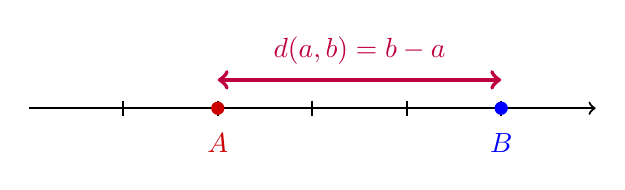
\begin{tikzpicture}[scale=1.2]
			\draw[->, thick] (-1,0) -- (5,0);
			\foreach \x in {0,1,2,3,4} { \draw[thick] (\x,0.08) -- (\x,-0.08); }
			\fill[red!80!black] (1,0) circle (2pt) node[below=2mm] {$A$};
			\fill[blue] (4,0) circle (2pt) node[below=2mm] {$B$};
			\draw[<->, line width=1.5pt, purple] (1,0.3) -- (4,0.3);
			\node[purple, above=2pt] at (2.5,0.3) {$d(a,b) = \abs{b - a}$};
		\end{tikzpicture}
	\end{center}
\end{df}

\begin{remarque}
	En particulier, pour tout réel $x$, la valeur absolue $\abs{x} = \abs{x - 0} = d(x,0)$ représente la \textbf{distance entre $x$ et l'origine $0$}.
\end{remarque}

\subsection{Équations et inéquations avec valeur absolue}

\begin{prop}[Résolution d'équations $\abs{x - a} = r$]
	Soient $a \in \R$ et $r \geqslant 0$.

	L'équation $\abs{x - a} = r$ signifie que la distance entre $x$ et $a$ est égale à $r$.
	\[
		\abs{x - a} = r \iff \begin{cases}x_1 = a - r \\ x_2 = a + r\end{cases}
	\]
\end{prop}

\newpage

\begin{ex}
	Résolvons dans $\R$ l'équation $\abs{x - 2} = 3$.

	\textbf{Interprétation :} On cherche les réels $x$ situés à une distance de $3$ du point d'abscisse $2$.

	\begin{center}
		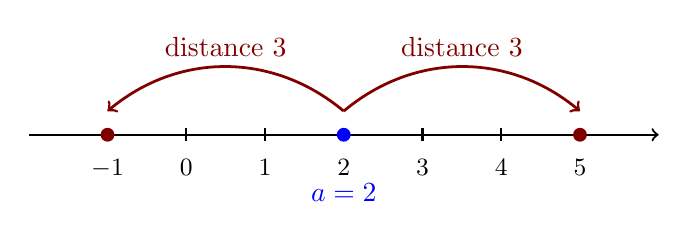
\begin{tikzpicture}[scale=1]
			\draw[->, thick] (-2,0) -- (6,0);
			\foreach \x in {-1,0,1,2,3,4,5} { \draw[thick] (\x,0.08) -- (\x,-0.08) node[below=1mm] {\small $\x$}; }
			\fill[blue] (2,0) circle (2.5pt) node[below=5mm] {$a = 2$};
			\draw[->, line width=1pt, red!50!black] (2,0.3) to[out=140,in=40] node[midway,above] {distance $3$} (-1,0.3);
			\draw[->, line width=1pt, red!50!black] (2,0.3) to[out=40,in=140] node[midway,above] {distance $3$} (5,0.3);
			\fill[red!50!black] (-1,0) circle (2.5pt);
			\fill[red!50!black] (5,0) circle (2.5pt);
		\end{tikzpicture}
	\end{center}

	L'ensemble des solutions est $S = \{-1 \,;\, 5\}$.
\end{ex}

\begin{prop}[Résolution d'inéquations $\abs{x - a} \leqslant r$]
	Soient $a \in \R$ et $r \geqslant 0$.

	L'inéquation $\abs{x - a} \leqslant r$ signifie que la distance entre $x$ et $a$ est inférieure ou égale à $r$.
	\begin{align*}
		\abs{x - a} \leqslant r & \iff x \in \intff{\pa{a - r}}{\pa{a + r}}        \\
		                        & \iff \pa{a - r} \leqslant x \leqslant \pa{a + r}
	\end{align*}
\end{prop}

\begin{ex}
	Résolvons dans $\R$ l'inéquation $\abs{x - 2} \leqslant 3$.

	\textbf{Interprétation :} On cherche les réels $x$ dont la distance à $2$ est inférieure ou égale à $3$.

	\begin{center}
		\begin{tikzpicture}[scale=1]
			\draw[->, thick] (-2.5,0) -- (6.5,0);
			\foreach \x in {-2,-1,0,1,3,4,5,6} { \draw[thick] (\x,0.08) -- (\x,-0.08) node[below=1mm] {\small $\x$}; }
			\draw[blue, line width=1.5pt, {Bracket[length=4pt, width=13pt]}-{Bracket[length=4pt, width=13pt]}] (-1.03,0) -- (5.03,0);
			\node[blue, above=6pt] at (2,0) {$\intff{-1}{5}$};
			\fill (2,0) circle (2pt) node[below=2mm] {$a = 2$};
			\draw[<->, thick, red!50!black] (-1,-1) -- (2,-1) node[midway,below] {$r=3$};
			\draw[<->, thick, red!50!black] (2,-1) -- (5,-1) node[midway,below] {$r=3$};
		\end{tikzpicture}
	\end{center}

	L'ensemble des solutions est l'intervalle $S = \intff{-1}{5}$.
\end{ex}



	\chapter{Équations et inéquations}

\section{Équations}

\subsection{Équations du premier degré}

\begin{methode}[Résoudre une équation du premier degré]
	Résoudre :
	\begin{multicols}{3}
		\begin{itemize}
			\item $-5x + 3 = -3x + 2$
			\item $3(x + 4) = -(x + 5) + 2$
		\end{itemize}
	\end{multicols}

	\begin{correction}
		\[
			\begin{array}{ll}%
				\def\arraystretch{1.2}%
				\begin{array}{rrcl}%
					     & -5x + 3  & = & -3x + 2                       \\
					\eqv & -5x + 3x & = & 2 - 3                         \\
					\eqv & -2x      & = & -1                            \\
					\eqv & x        & = & \dfrac{-1}{-2} = \dfrac{1}{2} \\
					     &          &   &
				\end{array} \qquad & \qquad %
				\def\arraystretch{1.2}%
				\begin{array}{rrcl}%
					     & 3(x + 4) & = & -(x + 5) + 2   \\
					\eqv & 3x + 12  & = & -x - 5 + 2     \\
					\eqv & 3x + x   & = & -12 - 5 + 2    \\
					\eqv & 4x       & = & -15            \\
					\eqv & x        & = & -\dfrac{15}{4}
				\end{array}%
			\end{array}%
		\]
	\end{correction}
\end{methode}

\subsection{Équation produit}

\begin{prop}[Règle du produit nul]
	Un produit de facteurs est nul \textbf{si et seulement si} l'un au moins de ses facteurs est nul.

	\[
		A \times B = 0 \iff A = 0 \quad \text{ou} \quad B = 0
	\]
\end{prop}

\begin{methode}[Résoudre une équation produit]
	Résoudre dans $\mathbb{R}$ :
	\begin{multicols}{3}
		\begin{itemize}
			\item $(4x + 6)(3 - 7x) = 0$
			\item $5x^2 - 4x = 0$
		\end{itemize}
	\end{multicols}

	\begin{correction}
		\nline
		\begin{itemize}
			\item $(4x + 6)(3 - 7x) = 0$

			      \[
				      \begin{array}{rcl}
					      (4x + 6)(3 - 7x) = 0 & \iff & \begin{cases}
						                                    4x + 6 = 0 \\
						                                    3 - 7x = 0
					                                    \end{cases} \iff \begin{cases}
						                                                     4x = -6 \\
						                                                     -7x = -3
					                                                     \end{cases} \iff \begin{cases}
						                                                                      x = \dfrac{-6}{4} = \dfrac{-3}{2} \\[3mm]
						                                                                      x = \dfrac{3}{7}
					                                                                      \end{cases} \\ %
					                           & \iff & S = \brac{\dfrac{-3}{2}\ ;\ \dfrac{3}{7}}
				      \end{array}
			      \]

			\item $5x^2 - 4x = 0$

			      On factorise par $x$ pour obtenir un produit.

			      \[
				      \begin{array}{rcl}
					      5x^2 - 4x = 0 & \iff & x(5x - 4) = 0 \iff \begin{cases}
						                                                x = 0 \\
						                                                5x - 4 = 0
					                                                \end{cases} \iff \begin{cases}
						                                                                 x = 0 \\
						                                                                 5x = 4
					                                                                 \end{cases} \iff \begin{cases}
						                                                                                  x = 0 \\[1mm]
						                                                                                  x = \dfrac{4}{5}
					                                                                                  \end{cases} \\[3mm] %
					                    & \iff & S = \brac{0\ ;\ \dfrac{4}{5}}
				      \end{array}
			      \]
		\end{itemize}
	\end{correction}
\end{methode}

\subsection{Équation quotient}

\begin{prop}[Règle du quotient nul]
	Un quotient est nul \textbf{si et seulement si} son numérateur est nul \textbf{et} son dénominateur est non nul.

	\[
		\dfrac{A}{B} = 0 \iff A = 0 \quad \text{et} \quad B \neq 0
	\]
\end{prop}

\begin{ex}
	Soit l'équation : $\quad\dfrac{x+2}{x+3} = 0$

	\begin{itemize}
		\item \textbf{Condition d'existence :} L'expression est définie pour $x + 3 \neq 0$, c'est-à-dire $x \neq -3$.
		\item \textbf{Résolution :} Pour tout $x \neq -3$,
		      \[
			      \dfrac{x+2}{x+3} = 0 \iff x + 2 = 0 \iff x = -2
		      \]
		\item \textbf{Conclusion :} Comme $-2 \neq -3$, la solution est $S = \{-2\}$.
	\end{itemize}
\end{ex}

\begin{methode}[Résoudre une équation quotient]
	Résoudre dans $\mathbb{R}$ :
	\begin{multicols}{3}
		\begin{enumerate}
			\item $\dfrac{3x+5}{x-1} = 0$
			\item $\dfrac{(2x+1)(x-3)}{x-4} = 0$
		\end{enumerate}
	\end{multicols}

	\begin{correction}
		\nline
		\begin{itemize}
			\item $\dfrac{3x+5}{x-1} = 0$
			      \[
				      \begin{array}{rcl}
					      \dfrac{3x+5}{x-1} = 0 & \iff & \begin{cases}
						                                     3x + 5 = 0 \\
						                                     x - 1 \neq 0
					                                     \end{cases} \iff \begin{cases}
						                                                      3x = -5 \\
						                                                      x \neq 1
					                                                      \end{cases} \iff \begin{cases}
						                                                                       x = -\dfrac{5}{3} \\[1mm]
						                                                                       x \neq 1
					                                                                       \end{cases} \\ %
					                            & \iff & S = \brac{-\dfrac{5}{3}}
				      \end{array}
			      \]

			\item $\dfrac{(2x+1)(x-3)}{x-4} = 0$
			      \[
				      \begin{array}{rcl}
					      \dfrac{(2x+1)(x-3)}{x-4} = 0 & \iff & \begin{cases}
						                                            (2x + 1)(x - 3) = 0 \\
						                                            x - 4 \neq 0
					                                            \end{cases} \iff \begin{cases}
						                                                             2x + 1 = 0 \\
						                                                             x - 3 = 0  \\
						                                                             x \neq 4
					                                                             \end{cases} \iff \begin{cases}
						                                                                              x = -\dfrac{1}{2} \\
						                                                                              x = 3             \\
						                                                                              x \neq 4
					                                                                              \end{cases} \\ %
					                                   & \iff & S = \brac{\dfrac{-1}{2} \,;\, 3}
				      \end{array}
			      \]
		\end{itemize}
	\end{correction}
\end{methode}

\subsection{Équation de la forme $x^2 = a$}

\begin{prop}[Solutions de $x^2 = a$]
	\nline
	\begin{itemize}
		\item Si $a < 0$ : l'équation n'a \textbf{pas de solution} dans $\mathbb{R}$.
		\item Si $a = 0$ : l'équation possède l'\textbf{unique solution} $x = 0$.
		\item Si $a > 0$ : l'équation possède \textbf{deux solutions} $x = -\sqrt{a}$ et $x = \sqrt{a}$.
	\end{itemize}
\end{prop}

\begin{demo}[Solutions de $x^2 = a$]
	\nline
	\begin{itemize}
		\item Si $a < 0$ : pas de solution car un carré est toujours positif.
		\item Si $a = 0$ : l'équation s'écrit $x^2 = 0$ donc $x = 0$.
		\item \textbf{Si $a > 0$ :} L'équation $x^2 = a$ admet deux solutions distinctes :
		      \[
			      \begin{array}{rcl}
				      x^2 = a & \iff & x^2 - a = 0                            \\[1mm]
				              & \iff & x^2 - \pa{\sqrt{a}}^2 = 0              \\[1mm]
				              & \iff & \pa{x - \sqrt{a}}\pa{x + \sqrt{a}} = 0 \\[2mm]
				              & \iff & \begin{cases}
					                       x - \sqrt{a} = 0 \\
					                       x + \sqrt{a} = 0
				                       \end{cases} \iff \begin{cases}
					                                        x = \sqrt{a} \\[1mm]
					                                        x = -\sqrt{a}
				                                        \end{cases}
			      \end{array}
		      \]
		      L'ensemble des solutions est donc $S = \brac{-\sqrt{a} \,;\, \sqrt{a}}$.
	\end{itemize}
\end{demo}

\begin{methode}[Résoudre une équation de la forme $x^2 = a$]
	Résoudre dans $\mathbb{R}$ :
	\begin{multicols}{3}
		\begin{itemize}
			\item $x^2 = 16$
			\item $x^2 = -8$
			\item $(x + 2)^2 = 9$
		\end{itemize}
	\end{multicols}

	\begin{correction}
		\nline
		\begin{itemize}
			\item $x^2 = 16$
			      \[
				      x^2 = 16
				      \iff \begin{cases}
					      x = -\sqrt{16} = -4 \\
					      x = \sqrt{16} = 4
				      \end{cases}
				      \iff S
				      = \{-4\ ;\ 4\}
			      \]

			\item $x^2 = -8$
			      \[
				      x^2 = -8 \iff S = \varnothing \quad \text{(un carré est toujours positif)}
			      \]

			\item $(x + 2)^2 = 9$
			      \[
				      (x + 2)^2 = 9
				      \iff \begin{cases}
					      x + 2 = -3 \\
					      x + 2 = 3
				      \end{cases}
				      \iff \begin{cases}
					      x = -5 \\
					      x = 1
				      \end{cases}
				      \iff S
				      = \{-5\ ;\ 1\}
			      \]
		\end{itemize}
	\end{correction}
\end{methode}

\section{Inéquations}

\subsection{Inéquations du premier degré}

\begin{defin}[Inéquation]
	Une \textbf{inéquation} est une inégalité contenant un nombre inconnu $x$.

	\textbf{Résoudre une inéquation}, c'est trouver toutes les valeurs de $x$ qui vérifient cette inégalité.

	Ces valeurs sont appelées les \textbf{solutions} de l'inéquation.
\end{defin}

\begin{ex}
	$2x + 1 > 4$ est une inéquation.

	Par exemple, $x = 10$ et $x = 2$ sont des solutions.
\end{ex}

\begin{attention}
	Lorsqu'on \textbf{multiplie} ou que l'on \textbf{divise} les deux membres d'une inéquation par un \textbf{nombre négatif}, on doit \textbf{changer le sens} de l'inégalité.
\end{attention}

\begin{ex}
	\[
		2 < 5 \quad \xrightarrow{\quad \text{multiplication par } -1 \quad} \quad - 2 > -5
	\]
\end{ex}

\newpage

\begin{methode}[Résoudre une inéquation du premier degré (1)]
	Résoudre et représenter les solutions sur une droite graduée :

	\[
		2x + 3 < 4 - 5x
	\]

	\begin{correction}
		\[
			\def\arraystretch{1.2}%
			\begin{array}{rrcl}%
				     & 2x + 3  & < & 4 - 5x       \\
				\iff & 2x + 5x & < & 4 - 3        \\
				\iff & 7x      & < & 1            \\
				\iff & x       & < & \dfrac{1}{7}
			\end{array}
		\]
		L'ensemble des solutions est $S = \intoo{-\infty}{\dfrac{1}{7}}$.

		\begin{center}
			\begin{tikzpicture}[xscale=4,yscale=0.5]
				\draw[-{Stealth[length=10pt, width=8pt]}, thick] (-0.5,0) -- (1.5,0);
				\foreach \x in {0,1} \draw[thick] (\x, -0.3) -- (\x, 0.3) node[below=8pt] {\x};
				\draw[red, line width=3pt, {-Bracket[reversed,width=15pt, length=5pt]}] (-0.5, 0) -- (1/7+0.05, 0);
				\node[above=8pt, red] at (1/7,0) {$\dfrac{1}{7}$};
			\end{tikzpicture}
		\end{center}
	\end{correction}
\end{methode}

\begin{methode}[Résoudre une inéquation du premier degré (2)]
	Résoudre et représenter les solutions sur une droite graduée :

	\[
		2(x - 4) \le 4x - 5
	\]

	\begin{correction}
		\[
			\def\arraystretch{1.2}%
			\begin{array}{rrcl}%
				     & 2(x - 4) & \le & 4x - 5                                                              \\
				\iff & 2x - 8   & \le & 4x - 5                                                              \\
				\iff & 2x - 4x  & \le & 8 - 5                                                               \\
				\iff & -2x      & \le & 3 \qquad \text{(division par } \pa{-2} \rarr \text{Le sens change)} \\
				\iff & x        & \ge & \dfrac{-3}{2}
			\end{array}
		\]
		L'ensemble des solutions est $S = \intfo{\dfrac{-3}{2}}{+\infty}$.

		\begin{center}
			\begin{tikzpicture}[xscale=1,yscale=0.5]
				\draw[-{Stealth[length=10pt, width=8pt]}, thick] (-4.5,0) -- (1.5,0);
				\foreach \x in {-4,-3,-2,-1,0,1} \draw[thick] (\x, -0.3) -- (\x, 0.3) node[below=8pt] {\x};
				\draw[red, line width=3pt, {Bracket[width=15pt, length=5pt]}-] (-1.5, 0) -- (1.5, 0);
				\node[above=8pt, red] at (-1.5,0) {$\dfrac{-3}{2}$};
			\end{tikzpicture}
		\end{center}
	\end{correction}
\end{methode}

\newpage

\subsection{Tableaux de signes}

\begin{defin}
	Un \textbf{tableau de signes} est un outil synthétique qui permet de visualiser immédiatement, selon les valeurs de l'inconnue $x$, si une expression mathématique est \textbf{positive} ($+$), \textbf{négative} ($-$) ou \textbf{nulle} ($0$).
\end{defin}

\begin{ex}{}
	Voici le tableau de signes d'une expression $A(x)$ définie sur $\mathbb{R}$ :
	\begin{center}
		\begin{tikzpicture}
			\tkzTabInit[lgt=2.5,espcl=2]{$x$ /1, $A(x)$ /1}{$-\infty$, $-1$, $4$, $+\infty$}
			\tkzTabLine{,-,z,+,z,-,}
		\end{tikzpicture}
	\end{center}

	L'expression $A(x)$ est strictement positive lorsque $x$ est compris entre $-1$ et $4$, c'est-à-dire pour $x \in ] - 1 \,;\, 4[$.

	\[
		A(x) \ge 0 \iff x \in \intff{-1}{4}
	\]

	Elle s'annule en $x = -1$ et $x = 4$.
\end{ex}

\begin{prop}[Signe de l'expression $ax + b$ (avec $a \neq 0$)]
	L'expression $ax + b$ s'annule pour $x = \frac{-b}{a}$.

	\begin{center}
		\begin{multicols}{2}
			\centering
			{$a > 0$}
			\vskip 2mm
			\begin{tikzpicture}
				\tkzTabInit[lgt=2,espcl=1.5]{$x$ /1, $ax + b$ /1}{$-\infty$, $\frac{-b}{a}$, $+\infty$}
				\tkzTabLine{,-,z,+,}
			\end{tikzpicture}

			\columnbreak

			\centering
			{$a < 0$}
			\vskip 2mm
			\begin{tikzpicture}
				\tkzTabInit[lgt=2,espcl=1.5]{$x$ /1, $ax + b$ /1}{$-\infty$, $\frac{-b}{a}$, $+\infty$}
				\tkzTabLine{,+,z,-,}
			\end{tikzpicture}
		\end{multicols}
	\end{center}
\end{prop}

\begin{demo}
	Pour déterminer le signe de $ax + b$ (avec $a \neq 0$), on cherche pour quelles valeurs de $x$ l'expression est strictement positive :
	\[
		ax + b > 0 \iff ax > -b
	\]
	Deux cas se présentent alors selon le signe du coefficient $a$ :

	\begin{itemize}
		\item \textbf{Si $a > 0$ :}

		      En divisant par $a$ sans changer le sens de l'inégalité, on obtient : $\quad x > \dfrac{-b}{a}$

		      L'expression $ax + b$ est donc strictement positive \textbf{après} $\dfrac{-b}{a}$ (et négative avant).

		\item \textbf{Si $a < 0$ :}

		      En divisant par $a$ (nombre négatif), le sens de l'inégalité change : $\quad x < \dfrac{-b}{a}$

		      L'expression $ax + b$ est donc strictement positive \textbf{avant} $\dfrac{-b}{a}$ (et négative après).
	\end{itemize}

	Ces résultats confirment la règle : l'expression $ax + b$ est du signe de $a$ après sa valeur d'annulation, ce qui valide les deux tableaux ci-dessus.
\end{demo}

\newpage

\begin{methode}[Tableau de signe d'une expression $ax + b$]
	Déterminer le tableau de signe de :
	\begin{multicols}{3}
		\begin{itemize}
			\item $2x + 6$
			\item $-3x + 12$
		\end{itemize}
	\end{multicols}
	\begin{correction}
		\nline
		\begin{multicols}{2}
			\begin{itemize}
				\item {Étude de $2x + 6$ :}
				      \[
					      \begin{aligned}
						      2x + 6 \ge 0 & \iff 2x \ge -6 \\
						                   & \iff x \ge -3
					      \end{aligned}
				      \]
				      L'expression est positive pour $x \ge -3$.

				      \begin{center}
					      \begin{tikzpicture}
						      \tkzTabInit[lgt=2.5,espcl=1.5]{$x$ /1, $2x + 6$ /1}{$-\infty$, $-3$, $+\infty$}
						      \tkzTabLine{,-,z,+,}
					      \end{tikzpicture}
				      \end{center}

				\item {Étude de $-3x + 12$ :}
				      \[
					      \begin{aligned}
						      -3x + 12 \ge 0 & \iff -3x \ge -12 \\
						                     & \iff x \le 4
					      \end{aligned}
				      \]
				      L'expression est positive pour $x \le 4$.

				      \begin{center}
					      \begin{tikzpicture}
						      \tkzTabInit[lgt=2.5,espcl=1.5]{$x$ /1, $-3x + 12$ /1}{$-\infty$, $4$, $+\infty$}
						      \tkzTabLine{,+,z,-,}
					      \end{tikzpicture}
				      \end{center}
			\end{itemize}
		\end{multicols}
	\end{correction}
\end{methode}

\begin{methode}[Tableau de signe d'un produit $(ax + b)(cx + d)$]
	Dresser le tableau de signe de :
	\[
		(3x - 9)(1 - 2x)
	\]

	\begin{correction}
		On étudie le signe de chaque facteur :
		\begin{multicols}{2}
			\begin{itemize}
				\item {Étude de $3x - 9$ :}
				      \[
					      \begin{aligned}
						      3x - 9 \ge 0 & \iff 3x \ge 9 \\
						                   & \iff x \ge 3
					      \end{aligned}
				      \]
				\item {Étude de $1 - 2x$ :}
				      \[
					      \begin{aligned}
						      1 - 2x \ge 0 & \iff -2x \ge -1         \\
						                   & \iff x \le \tfrac{1}{2}
					      \end{aligned}
				      \]
			\end{itemize}
		\end{multicols}

		\begin{center}
			\begin{tikzpicture}
				\tkzTabInit[lgt=4,espcl=2]
				{$x$ /1, $3x - 9$ /1, $1 - 2x$ /1, $(3x - 9)(1 - 2x)$ /1}
				{$-\infty$, $\frac{1}{2}$, $3$, $+\infty$}
				\tkzTabLine{,-,,-,z,+,}
				\tkzTabLine{,+,z,-,,-,}
				\tkzTabLine{,-,z,+,z,-,}
			\end{tikzpicture}
		\end{center}
		\textit{On applique la règle des signes pour déterminer le signe du produit.}
	\end{correction}
\end{methode}

\subsection{Inéquation produit}

\begin{methode}[Résoudre une inéquation produit]
	Résoudre dans $\mathbb{R}$ :
	\[
		(3 - 6x)(x + 2) > 0
	\]

	\begin{correction}
		Établissons le tableau de signe de $(3 - 6x)(x + 2)$ :

		\begin{multicols}{2}
			\begin{itemize}
				\item \textbf{Étude de $3 - 6x$ :}
				      \[
					      \begin{aligned}
						      3 - 6x \ge 0 & \iff -6x \ge -3         \\
						                   & \iff x \le \tfrac{1}{2}
					      \end{aligned}
				      \]

				\item \textbf{Étude de $x + 2$ :}
				      \[
					      \begin{aligned}
						      x + 2 \ge 0 & \iff x \ge -2
					      \end{aligned}
				      \]
			\end{itemize}
		\end{multicols}
		\begin{center}
			\begin{tikzpicture}
				\tkzTabInit[lgt=4,espcl=2]
				{$x$ /1, $3 - 6x$ /1, $x + 2$ /1, $(3 - 6x)(x + 2)$ /1}
				{$-\infty$, $-2$, $\tfrac{1}{2}$, $+\infty$}
				\tkzTabLine{,+,,+,z,-,}
				\tkzTabLine{,-,z,+,,+,}
				\tkzTabLine{,-,z,+,z,-,}
			\end{tikzpicture}
		\end{center}

		On veut que le produit soit strictement positif ($> 0$).
		\[
			S = \intoo{-2}{\tfrac{1}{2}}
		\]
	\end{correction}
\end{methode}

\subsection{Inéquation quotient}

\begin{methode}[Résoudre une inéquation quotient]
	Résoudre dans $\mathbb{R}$ :

	\[
		\dfrac{2-6x}{3x-2} \le 0
	\]

	\begin{correction}
		\nline
		\begin{itemize}
			\item \textbf{Numérateur :}
			      \[
				      2 - 6x \ge 0 \iff x \le \frac{1}{3}
			      \]
			\item \textbf{Dénominateur :}
			      \[
				      3x - 2 \ge 0 \iff x \ge \frac{2}{3}
			      \]
			\item \textbf{Valeur interdite :}
			      \[
				      3x - 2 = 0 \iff x = \frac{2}{3}
			      \]
		\end{itemize}

		\begin{center}
			\tikzset{double style/.style={double, double distance=3pt, thick}}
			\begin{tikzpicture}
				\tkzTabInit[lgt=4,espcl=2]
				{$x$ /1, $2 - 6x$ /1, $3x - 2$ /1, $\dfrac{2-6x}{3x-2}$ /1}
				{$-\infty$, $\tfrac{1}{3}$, $\tfrac{2}{3}$, $+\infty$}
				\tkzTabLine{,+,z,-,,-,}
				\tkzTabLine{,-,,-,z,+,}
				\tkzTabLine{,-,z,+,d,-,}
			\end{tikzpicture}
		\end{center}

		On veut que le quotient soit inférieur ou égal à zéro ($\le 0$).
		\[
			S = \intof{-\infty}{\dfrac{1}{3}} \cup \intoo{\dfrac{2}{3}}{+\infty}
		\]
	\end{correction}
    %
	% \newpage
    %
	% \textbf{Interprétation graphique}
    %
	% \begin{center}
	% 	\begin{tikzpicture}[xscale=3,yscale=1.2]
	% 		\def\xmin{-1.2} \def\xmax{1.8}
	% 		\def\ymin{-5} \def\ymax{3}
    %
	% 		\draw[black!10, very thin, step=0.5] (\xmin,\ymin+0.1) grid (\xmax,\ymax-0.1);
	% 		\draw[->, >=Stealth, thick] (\xmin, 0) -- (\xmax, 0) node[right] {$x$};
	% 		\draw[->, >=Stealth, thick] (0, \ymin) -- (0, \ymax) node[above] {$y$};
    %
	% 		\draw[dashed, thick, blue!40] (2/3, \ymin) -- (2/3, \ymax) node[above, black, font=\small] {$x = \dfrac{2}{3}$};
	% 		\draw[dashed, thick, blue!40] (\xmin, -2) -- (\xmax, -2);
    %
	% 		\foreach \x in {-1, 1} \draw (\x, 0.1) -- (\x, -0.1) node[below, font=\small] {$\x$};
	% 		\foreach \y in {-4, -2, 2} \draw (0.05, \y) -- (-0.05, \y) node[left, font=\small] {$\y$};
	% 		\node[below left, font=\small] at (0,0) {0};
    %
	% 		\begin{scope}
	% 			\clip (\xmin, \ymin) rectangle (\xmax, \ymax);
	% 			\draw[thick, blue, samples=200, domain=\xmin:0.62] plot (\x, {(2-6*\x)/(3*\x-2)});
	% 			\draw[thick, blue, samples=200, domain=0.72:\xmax] plot (\x, {(2-6*\x)/(3*\x-2)});
	% 		\end{scope}
    %
	% 		\node[circle, fill=red, inner sep=1.8pt] at (1/3, 0) {};
	% 		\node[below, red, yshift=-5pt, xshift=2mm] at (1/3, 0) {$\dfrac{1}{3}$};
    %
	% 		\draw[line width=2.5pt, red] (\xmin, 0) -- (1/3, 0);
	% 		\draw[line width=2.5pt, red] (2/3, 0) -- (\xmax, 0);
	% 	\end{tikzpicture}
	% \end{center}
\end{methode}

	\part{Statistiques et probabilités}
	\input{tex/2nde/proportion}
	\input{tex/2nde/statistiques}
	\input{tex/2nde/probabilites}
	\input{tex/2nde/probabilite-conditionnelle}
	\part{Fonctions}
	\input{tex/2nde/generalites-sur-les-fonctions}
	\input{tex/2nde/variations-extremums}
	\input{tex/2nde/fonctions-affines}
	\input{tex/2nde/fonctions-de-reference}
	\part{Géométrie}
	\input{tex/2nde/notion-de-vecteurs}
	\input{tex/2nde/reperage-dans-le-plan}
	\chapter{Vecteurs et repérage}

\section{Repère du plan}

\begin{defin}[Repère du plan]
	On appelle \textbf{repère du plan} tout triplet $\vOIJ$ où $O$ est un point et $\vec{i}$, $\vec{j}$ sont deux vecteurs non colinéaires.

	Si $\vec{i} = \vec{OI}$ et $\vec{j} = \vec{OJ}$, ce repère se note aussi $\OIJ$.

	\begin{itemize}
		\item Un repère est dit \textbf{orthogonal} si $\vec{i}$ et $\vec{j}$ ont des directions perpendiculaires.
		\item Un repère est dit \textbf{orthonormé} s'il est orthogonal et si $\vec{i}$ et $\vec{j}$ sont de norme $1$.
	\end{itemize}

	\begin{center}
		\begin{tikzpicture}[scale=0.9, >=Stealth]
			\def\lenAxis{1.5}\def\lenVector{0.8}\def\lenTextWidth{2.5cm}
			\begin{scope}[shift={(0,0)}]
				\draw[->] (-\lenAxis,0) -- (\lenAxis+0.3,0);
				\draw[->] ({-\lenAxis*0.4}, {-\lenAxis*1.2}) -- ({\lenAxis*0.4}, {\lenAxis*1.2});
				\coordinate (O) at (0,0);
				\draw[->, thick, blue] (O) -- (\lenVector,0) node[midway, below] {$\vec{i}$};
				\draw[->, thick, blue] (O) -- ({\lenVector*0.6}, {\lenVector*1.8}) node[midway, left] {$\vec{j}$};
				\node[below left] at (O) {$O$};
				\node[fill=white, align=center, text width=\lenTextWidth, font=\small, anchor=north west] at (-\lenAxis, -\lenAxis-0.5) {Repère\\quelconque};
			\end{scope}
			\begin{scope}[shift={(5,0)}]
				\draw[->] (-\lenAxis,0) -- (\lenAxis+0.3,0);
				\draw[->] (0, -\lenAxis) -- (0, \lenAxis+0.3);
				\coordinate (O) at (0,0);
				\draw[->, thick, blue] (O) -- (\lenVector,0) node[midway, below] {$\vec{i}$};
				\draw[->, thick, blue] (O) -- (0, {\lenVector*1.6}) node[midway, left] {$\vec{j}$};
				\node[below left] at (O) {$O$};
				\node[fill=white, align=center, text width=\lenTextWidth, font=\small, anchor=north west] at (-\lenAxis, -\lenAxis-0.5) {Repère\\orthogonal};
			\end{scope}
			\begin{scope}[shift={(10,0)}]
				\draw[->] (-\lenAxis,0) -- (\lenAxis+0.3,0);
				\draw[->] (0, -\lenAxis) -- (0, \lenAxis+0.3);
				\coordinate (O) at (0,0);
				\draw[->, thick, blue] (O) -- (\lenVector,0) node[midway, below] {$\vec{i}$};
				\draw[->, thick, blue] (O) -- (0, \lenVector) node[midway, left] {$\vec{j}$};
				\node[below left] at (O) {$O$};
				\node[fill=white, align=center, text width=\lenTextWidth, font=\small, anchor=north west] at (-\lenAxis, -\lenAxis-0.5) {Repère\\orthonormé};
			\end{scope}
		\end{tikzpicture}
	\end{center}
\end{defin}

\section{Coordonnées d'un vecteur}

\begin{defin}{Coordonnées d'un vecteur}
	Soit $(O, \vv{i}, \vv{j})$ un repère du plan et $\vv{u}$ un vecteur.

	Il existe un unique couple de nombres réels $(x\,;\,y)$ tel que :
	\[
		\vv{u} = x\vv{i} + y\vv{j}
	\]

	Le nombre $x$ est l'\textbf{abscisse} du vecteur $\vv{u}$ et $y$ est son \textbf{ordonnée}.

	On note $\vv{u}\coord{x}{y}$ ou $\vv{u}(x\,;\,y)$.
\end{defin}

\begin{ex}{}
	Pour aller de $A$ vers $B$, on parcourt un chemin : 3 unités vers la droite et 2 unités vers le haut.

	Ainsi $\vec{AB} = 3\vec{i} + 2\vec{j}$. Les coordonnées de $\vec{AB}$ se notent $\coord{3}{2}$ ou $(3\,;\,2)$.

	\begin{center}
		\begin{tikzpicture}[scale=0.9, >=Stealth]
			\draw[help lines, gray!50] (-1,-1) grid (7,4);
			\def\lenAxisX{7}\def\lenAxisY{4}
			\def\refLenVector{1}
			\coordinate (O) at (0,0);
			\draw[thick, ->] (-1,0) -- (\lenAxisX,0);
			\draw[thick, ->] (0,-1) -- (0,\lenAxisY);
			\node[below left] at (O) {$O$};
			\foreach \x in {1,2,3,4,5,6} { \draw (\x,2pt) -- (\x,-2pt); }
			\foreach \y in {1,2,3} { \draw (2pt,\y) -- (-2pt,\y); }
			\draw[->, ultra thick, green!50!black] (O) -- (\refLenVector,0) node[midway, below] {$\vec{i}$};
			\draw[->, ultra thick, red] (O) -- (0,\refLenVector) node[midway, left] {$\vec{j}$};
			\coordinate (A) at (2,1);
			\coordinate (Corner) at (5,1);
			\coordinate (B) at (5,3);
			\node[anchor=east, fill=white] at (A) {$A$};
			\node[anchor=south,above right] at (B) {$B$};
			\draw[->, thick, green!50!black, dashed] (A) -- (3,1);
			\draw[->, thick, green!50!black, dashed] (3,1) -- (4,1);
			\draw[->, thick, green!50!black, dashed] (4,1) -- (Corner);
			\node[green!50!black, below, fill=white] at ($(A)!0.5!(Corner)+(0,-0.1)$) {$3\vec{i}$};
			\draw[->, thick, red, dashed] (Corner) -- (5,2);
			\draw[->, thick, red, dashed] (5,2) -- (B);
			\node[red, right, fill=white] at ($(Corner)!0.5!(B)+(0.1,0)$) {$2\vec{j}$};
			\draw[->, thick, black] (A) -- (B) node[midway, above, sloped, fill=white] {$3\vec{i}+2\vec{j}$};
			\fill[black] (A) circle (2pt);
			\fill[black] (B) circle (2pt);
			\fill[black] (Corner) circle (2pt);
		\end{tikzpicture}
	\end{center}
\end{ex}

\begin{methode}[Déterminer les coordonnées d'un vecteur par lecture graphique]
	Dans le repère $\vOIJ$, placer les points :
	\begin{multicols}{4}
		\begin{itemize}
			\item $C\coordl{-1}{-2}$
			\item $D\coordl{-2}{3}$
			\item $E\coordl{1}{-4}$
			\item $F\coordl{4}{-2}$
		\end{itemize}
	\end{multicols}

	Déterminer, par lecture graphique, les coordonnées des vecteurs $\vec{CD}$ et $\vec{EF}$.

	\begin{center}
		\begin{tikzpicture}[scale=0.8, >=Stealth]
			\draw[thin, gray!30] (-3.5,-4.5) grid (5.5,3.5);
			\draw[->, thick] (-3.5,0) -- (5.5,0) node[right] {$x$};
			\draw[->, thick] (0,-4.5) -- (0,3.5) node[above] {$y$};
			\coordinate (O) at (0,0);
			\node[below left] at (O) {$O$};
			\draw[->, ultra thick, blue] (O) -- (1,0) node[midway, below] {$\vec{i}$};
			\draw[->, ultra thick, blue] (O) -- (0,1) node[midway, left] {$\vec{j}$};
			\coordinate (C) at (-1,-2);
			\coordinate (D) at (-2,3);
			\coordinate (E) at (1,-4);
			\coordinate (F) at (4,-2);
			\draw[->, ultra thick, green!50!black, dotted] (C) -- (-2,-2) node[midway, below] {$-\vec{i}$};
			\draw[->, ultra thick, green!50!black, dotted] (-2,-2) -- (D) node[midway, left] {$5\vec{j}$};
			\draw[->, ultra thick, green!50!black, dotted] (E) -- (4,-4) node[midway, below] {$3\vec{i}$};
			\draw[->, ultra thick, green!50!black, dotted] (4,-4) -- (F) node[midway, right, fill=white] {$2\vec{j}$};
			\draw[->, ultra thick, black] (C) -- (D);
			\draw[->, ultra thick, black] (E) -- (F);
			\fill[black] (C) circle (3pt) node[right] {$C$};
			\fill[black] (D) circle (3pt) node[above] {$D$};
			\fill[black] (E) circle (3pt) node[left] {$E$};
			\fill[black] (F) circle (3pt) node[right] {$F$};
		\end{tikzpicture}
	\end{center}

	\begin{correction}
		\nline
		\begin{multicols}{2}
			\begin{itemize}
				\item $\vec{CD} = -\vec{i} + 5\vec{j}$ \quad donc $\vec{CD}\coord{-1}{5}$
				\item $\vec{EF} = 3\vec{i} + 2\vec{j}$ \quad donc $\vec{EF}\coord{3}{2}$
			\end{itemize}
		\end{multicols}
	\end{correction}
\end{methode}

\begin{prop}[Coordonnées d'un vecteur $\vec{AB}$]
	\nline
	\begin{wrapstuff}[r]
		\begin{tikzpicture}[scale=0.9, >=Stealth]
			\draw[->, thick] (-0.5,0) -- (6.8,0) node[right] {\footnotesize $x$};
			\draw[->, thick] (0,-0.5) -- (0,4.8) node[right] {\footnotesize $y$};
			\node[below left, font=\small] at (0,0) {$O$};
			\draw[->, ultra thick, blue] (0,0) -- (1,0) node[midway, below] {$\vv{i}$};
			\draw[->, ultra thick, blue] (0,0) -- (0,1) node[midway, left] {$\vv{j}$};
			\coordinate (A) at (1.5,1.8);
			\coordinate (B) at (5,4);
			\coordinate (C) at (5,1.8);
			\draw[dotted, gray!20!black] (1.5,0) node[below, font=\small] {$x_A$} -- (A) -- (0,1.8) node[left, font=\small] {$y_A$};
			\draw[dotted, gray!20!black] (5,0) node[below, font=\small] {$x_B$} -- (C) -- (B) -- (0,4) node[left, font=\small] {$y_B$};
			\draw[->, ultra thick, green!50!black, dashed] (A) -- (C) node[midway, below, font=\small] {$(x_B - x_A)\vv{i}$};
			\draw[->, ultra thick, red, dashed] (C) -- (B) node[midway, right, font=\small] {$(y_B - y_A)\vv{j}$};
			\draw[->, ultra thick, blue!80!black] (A) -- (B) node[midway, above, sloped, fill=white] {$\vv{AB}\coord{x_B - x_A}{y_B - y_A}$};
			\fill[black] (A) circle (2.2pt) node[above left] {$A$};
			\fill[black] (B) circle (2.2pt) node[above left] {$B$};
		\end{tikzpicture}
	\end{wrapstuff}

	Soit deux points $A\coordl{x_A}{y_A}$ et $B\coordl{x_B}{y_B}$.

	Le vecteur $\vec{AB}$ a pour coordonnées :
	\[
		\vec{AB}\coord{x_B - x_A}{y_B - y_A}
	\]

	\rule{0mm}{23mm}
\end{prop}

\begin{methode}[Déterminer les coordonnées d'un vecteur par calcul]
	Calculer les coordonnées des vecteurs $\vec{AB}$, $\vec{CD}$ et $\vec{EF}$ avec :
	\begin{multicols}{3}
		\begin{itemize}
			\item $A\coordl{2}{1}$
			\item $B\coordl{5}{3}$
			\item $C\coordl{-1}{-2}$
			\item $D\coordl{-2}{3}$
			\item $E\coordl{1}{-4}$
			\item $F\coordl{4}{-2}$.
		\end{itemize}
	\end{multicols}

	\begin{correction}
		\[
			\begin{array}{lllll}
				\begin{array}{rcl} \vec{AB} & = & \coord{x_B-x_A}{y_B-y_A} \\ & = & \coord{5-2}{3-1} = \coord{3}{2} \end{array}         & \qquad
				\begin{array}{rcl} \vec{CD} & = & \coord{x_D-x_C}{y_D-y_C} \\ & = & \coord{-2-(-1)}{3-(-2)} = \coord{-1}{5} \end{array} & \qquad
				\begin{array}{rcl} \vec{EF} & = & \coord{x_F-x_E}{y_F-y_E} \\ & = & \coord{4-1}{-2-(-4)} = \coord{3}{2} \end{array}
			\end{array}
		\]
	\end{correction}
\end{methode}

\begin{prop}[Opérations sur les coordonnées]
	Soit deux vecteurs $\vec{u}\coord{x}{y}$, $\vec{v}\coord{x'}{y'}$ et un réel $k$.

	On a :
	\[
		\vec{u} + \vec{v} \coord{x+x'}{y+y'}
		\qquad
		k\vec{u} \coord{kx}{ky}
		\qquad
		-\vec{u} \coord{-x}{-y}
	\]

	De plus, $\vec{u}$ et $\vec{v}$ sont égaux si et seulement si $x = x'$ et $y = y'$.
\end{prop}

\begin{methode}[Appliquer les formules sur les coordonnées de vecteurs]
	Considérant $\vec{AB}\coord{3}{2}$ et $\vec{CD}\coord{-1}{5}$, calculer les coordonnées des vecteurs $3\vec{AB}$, $4\vec{CD}$ et $3\vec{AB} - 4\vec{CD}$.

	\begin{correction}
		\nline
		\begin{multicols}{2}
			\begin{itemize}[label=]
				\item $\begin{array}{rcl} 3\vec{AB} & = & \coord{3\times3}{3\times2} = \coord{9}{6} \end{array}$
				\item $\begin{array}{rcl} 4\vec{CD} & = & \coord{4\times(-1)}{4\times5} = \coord{-4}{20} \end{array}$
				\item $\begin{array}{rcl} 3\vec{AB} - 4\vec{CD} & = & \coord{9-(-4)}{6-20} = \coord{13}{-14} \end{array}$
			\end{itemize}
		\end{multicols}
	\end{correction}
\end{methode}

\begin{methode}[Calculer les coordonnées d'un point défini par une égalité vectorielle]
	Soit $A\coordl{1}{2}$, $B\coordl{-4}{3}$ et $C\coordl{1}{-2}$.

	Déterminer les coordonnées du point $D$ tel que $ABCD$ soit un parallélogramme.

	\begin{correction}
		$ABCD$ est un parallélogramme $\iff \vec{AB} = \vec{DC}$.

		On pose $D\coordl{x_D}{y_D}$.

		On a :
		\[
			\vec{AB}\coord{-4-1}{3-2} = \coord{-5}{1}\quad\text{ et }\quad\vec{DC}\coord{1-x_D}{-2-y_D}
		\]

		On en déduit :
		\begin{align*}
			\vec{AB} = \vec{DC} & \iff \begin{cases} 1 - x_D = -5 \\ -2 - y_D = 1 \end{cases}                                                     \\
			                    & \iff \begin{cases} -x_D = -5 - 1 \\ -y_D = 1 + 2 \end{cases} \iff \begin{cases} x_D = 6 \\ y_D = -3 \end{cases}
		\end{align*}

		Les coordonnées du point $D$ sont donc $\coord{6}{-3}$.
	\end{correction}
\end{methode}

\section{Colinéarité de deux vecteurs}

\subsection{Critère de colinéarité}

\begin{prop}[Critère de colinéarité]
	Soit $\vec{u}\coord{x}{y}$ et $\vec{v}\coord{x'}{y'}$.

	Dire que $\vec{u}$ et $\vec{v}$ sont colinéaires revient à dire que :
	\[
		xy' - yx' = 0
	\]
\end{prop}

\begin{remarque}
	Dire que $\vec{u}$ et $\vec{v}$ sont colinéaires revient à dire que les coordonnées des deux vecteurs sont proportionnelles, c'est-à-dire $xy' = yx'$.
\end{remarque}

\begin{demo}[Condition de colinéarité]
	\nline
	\begin{itemize}
		\item Si l'un des vecteurs est nul, l'équivalence est évidente.
		\item Supposons maintenant que les vecteurs $\vec{u}$ et $\vec{v}$ soient non nuls.
		      \begin{itemize}[itemsep=2mm]
			      \item Dire que les vecteurs $\vec{u}\coord{x}{y}$ et $\vec{v}\coord{x'}{y'}$ sont colinéaires équivaut à dire qu'il existe $k\in\R$ tel que :
			            \[
				            \vec{u} = k\vec{v}
			            \]

			            Les coordonnées des vecteurs $\vec{u}$ et $\vec{v}$ sont donc proportionnelles, ce qui correspond au tableau de proportionnalité suivant :

			            \begin{center}
				            \def\arraystretch{1.4}
				            \begin{tabular}{|l|c|c|} \hline
					            \text{abscisse} & $x$ & $x'$ \\ \hline
					            \text{ordonnée} & $y$ & $y'$ \\ \hline
				            \end{tabular}
			            \end{center}

			            D'après le produit en croix, on a $xy' = yx'$, soit encore $xy' - yx' = 0$.

			      \item Réciproquement, supposons que $xy' - yx' = 0$.

			            Le vecteur $\vec{v}$ étant non nul, l'une de ses coordonnées est non nulle.

			            Supposons que $x' \neq 0$ et posons alors $k = \dfrac{x}{x'}$.

			            L'égalité $xy' - yx' = 0$ s'écrit alors :
			            \begin{align*}
				            xy' - yx' = 0 & \iff  yx' = xy'                                    \\
				                          & \iff  y = \frac{x y'}{x'} = \frac{x}{x'} y' = k y'
			            \end{align*}

			            Comme on a déjà $x = k x'$ par définition de $k$, on en déduit que $\vec{u} = k\vec{v}$.

			            Les vecteurs $\vec{u}$ et $\vec{v}$ sont donc colinéaires.
		      \end{itemize}
	\end{itemize}
\end{demo}

\begin{methode}[Vérifier si deux vecteurs sont colinéaires]
	Dans chaque cas, vérifier si les vecteurs $\vec{u}$ et $\vec{v}$ sont colinéaires :
	\begin{multicols}{3}
		\begin{enumerate}
			\item $\vec{u}\coord{4}{-7}\ \text{ et }\ \vec{v}\coord{-12}{21}$
			\item $\vec{u}\coord{5}{-2}\ \text{ et }\ \vec{v}\coord{15}{-7}$
		\end{enumerate}
	\end{multicols}

	\begin{correction}
		\nline
		\begin{enumerate}[itemsep=2mm]
			\item $\vec{u}\coord{4}{-7}\ \text{ et }\ \vec{v}\coord{-12}{21}$
			      \[
				      \def\arraystretch{1.2}\begin{array}{rcl} xy' - yx' & = & 4\times 21 - (-7)\times(-12)\\ & = & 84 - 84 = 0\end{array}
			      \]

			      Le critère est vérifié, donc $\vec{u}$ et $\vec{v}$ sont colinéaires.

			      On peut également observer directement que $\vec{v} = -3\vec{u}$.

			\item $\vec{u}\coord{5}{-2}\ \text{ et }\ \vec{v}\coord{15}{-7}$
			      \[
				      \def\arraystretch{1.2} \begin{array}{rcl} xy' - yx' & = & 5\times(-7) - (-2)\times 15 \\ & = & -35 + 30 = -5 \neq 0 \end{array}
			      \]

			      Le critère n'est pas vérifié, donc $\vec{u}$ et $\vec{v}$ ne le sont pas.
		\end{enumerate}
	\end{correction}
\end{methode}

\subsection{Déterminant de deux vecteurs}

\begin{defin}[Déterminant]
	Soit $\vec{u}\coord{x}{y}$ et $\vec{v}\coord{x'}{y'}$.

	Le nombre $xy' - yx'$ est appelé \textbf{déterminant} des vecteurs $\vec{u}$ et $\vec{v}$.

	On note :
	\[
		\det(\vec{u}\,;\,\vec{v}) = \determinant{x & x' \\ y & y'} = xy' - yx'
	\]
\end{defin}

\begin{prop}
	Soient $\vec{u}$ et $\vec{v}$, deux vecteurs non nuls. On a :
	\[
		\vec{u}\ \text{ et }\ \vec{v}\ \text{colinéaires}\ \iff\ \det(\vec{u}\,;\,\vec{v}) = 0
	\]
\end{prop}

\begin{methode}[Vérifier si deux vecteurs sont colinéaires à l'aide du déterminant]
	Dans chaque cas, vérifier si les vecteurs $\vec{u}$ et $\vec{v}$ sont colinéaires :
	\begin{multicols}{3}
		\begin{enumerate}
			\item $\vec{u}\coord{-6}{10}\quad\text{et}\quad\vec{v}\coord{9}{-15}$
			\item $\vec{u}\coord{4}{9}\quad\text{et}\quad\vec{v}\coord{11}{23}$
		\end{enumerate}
	\end{multicols}

	\begin{correction}
		\nline
		\begin{enumerate}[itemsep=2mm]
			\item $\vec{u}\coord{-6}{10}\quad\text{et}\quad\vec{v}\coord{9}{-15}$
			      \[
				      \def\arraystretch{1.2}
				      \begin{array}{rclll}
					      \det(\vec{u}\,;\,\vec{v}) & = & \determinant{-6              & 9             \\ 10 & -15} & \\
					                                & = & (-6)\times(-15) - 10\times 9 & = 90 - 90 = 0
				      \end{array}
			      \]

			      Les vecteurs $\vec{u}$ et $\vec{v}$ sont colinéaires.

			\item $\vec{u}\coord{4}{9}\quad\text{et}\quad\vec{v}\coord{11}{23}$
			      \[
				      \def\arraystretch{1.2}
				      \begin{array}{rcll}
					      \det(\vec{u}\,;\,\vec{v}) & = & \determinant{4         & 11                    \\ 9 & 23} & \\
					                                & = & 4\times23 - 9\times 11 & = 92 - 99 = -7 \neq 0
				      \end{array}
			      \]

			      Les vecteurs $\vec{u}$ et $\vec{v}$ ne sont pas colinéaires.
		\end{enumerate}
	\end{correction}
\end{methode}

\subsection{Applications}

\begin{prop}[Parallélisme et alignement]
	\nline
	\begin{itemize}
		\item Dire que les droites $(AB)$ et $(CD)$ sont parallèles revient à dire que les vecteurs $\vec{AB}$ et $\vec{CD}$ sont colinéaires.
		\item Dire que les points $A$, $B$ et $C$ sont alignés revient à dire que les vecteurs $\vec{AB}$ et $\vec{AC}$ sont colinéaires.
	\end{itemize}
\end{prop}

\begin{methode}[Appliquer la colinéarité]
	On considère les points :
	\begin{multicols}{3}
		\begin{itemize}
			\item $A\coordl{-1}{1}$
			\item $B\coordl{3}{2}$
			\item $C\coordl{-2}{-3}$
			\item $D\coordl{6}{-1}$
			\item $E\coordl{5}{0}$
		\end{itemize}
	\end{multicols}

	\begin{enumerate}
		\item Démontrer que les droites $(AB)$ et $(CD)$ sont parallèles.
		\item Démontrer que les points $E$, $B$ et $D$ sont alignés.
	\end{enumerate}

	\begin{correction}
		\nline
		\begin{enumerate}[itemsep=4mm]
			\item On calcule les coordonnées de $\vec{AB}$ et $\vec{CD}$ :
			      \[
				      \vec{AB}\coord{3-(-1)}{2-1} = \coord{4}{1}
				      \qquad\text{et}\qquad
				      \vec{CD}\coord{6-(-2)}{-1-(-3)} = \coord{8}{2}
			      \]

			      On a :
			      \[
				      \def\arraystretch{1.4}
				      \begin{array}{rcl}
					      \det(\vec{AB}\,;\,\vec{CD}) & = & \determinant{4                  & 8 \\ 1 & 2}\\
					                                  & = & 4\times2 - 8\times1 = 8 - 8 = 0
				      \end{array}
			      \]

			      Les vecteurs $\vec{AB}$ et $\vec{CD}$ sont colinéaires, donc les droites $(AB)$ et $(CD)$ sont parallèles.

			\item On calcule les coordonnées de $\vec{EB}$ et $\vec{ED}$ :
			      \[
				      \vec{EB}\coord{3-5}{2-0} = \coord{-2}{2}
				      \qquad\text{et}\qquad
				      \vec{ED}\coord{6-5}{-1-0} = \coord{1}{-1}
			      \]

			      On a :
			      \[
				      \def\arraystretch{1.4}
				      \begin{array}{rcl}
					      \det(\vec{EB}\,;\,\vec{ED}) & = & \determinant{-2                       & 1 \\ 2 & -1}\\
					                                  & = & (-2)\times(-1) - 2\times1 = 2 - 2 = 0
				      \end{array}
			      \]

			      Les vecteurs $\vec{EB}$ et $\vec{ED}$ sont colinéaires, donc les points $E$, $B$ et $D$ sont alignés.
		\end{enumerate}

		\begin{center}
			\begin{tikzpicture}[scale=1.4, >=Stealth]
				\clip (-2.5,-3.5) rectangle (8.5,3.7);
				\draw[thin, gray!50] (-2.5,-3.5) grid (7.5,3.5);
				\draw[->, thick] (-3.5,0) -- (7.5,0) node[right] {\footnotesize $x$};
				\draw[->, thick] (0,-3.5) -- (0,3.5) node[right] {\footnotesize $y$};
				\node[below left, font=\small] at (0,0) {$O$};
				\draw[->, ultra thick, blue] (0,0) -- (1,0) node[midway, below] {$\vv{i}$};
				\draw[->, ultra thick, blue] (0,0) -- (0,1) node[midway, left] {$\vv{j}$};
				\coordinate (A) at (-1,1);
				\coordinate (B) at (3,2);
				\coordinate (C) at (-2,-3);
				\coordinate (D) at (6,-1);
				\coordinate (E) at (5,0);
				\fill[black] (0,0) circle (2pt);
				% \draw[->, thick] (0,-3.5) -- (0,3.5);
				\fill[black] (A) circle (2pt) node[above=1mm, fill=white] {$A$};
				\fill[black] (B) circle (2pt) node[above=1mm, fill=white] {$B$};
				\fill[black] (C) circle (2pt) node[below=1mm, fill=white] {$C$};
				\fill[black] (D) circle (2pt) node[below=1mm, fill=white] {$D$};
				\fill[black] (E) circle (2pt) node[above right, fill=white] {$E$};
				\draw[thick, blue!80!black, domain=-2.5:6.5] plot (\x, {0.25*\x + 1.25}) node[right, fill=white] {$(AB)$};
				\draw[thick, blue!80!black, domain=-2.5:7.2] plot (\x, {0.25*\x - 2.5}) node[right, fill=white] {$(CD)$};
				\draw[thick, red!80!black, domain=-1.5:7.2] plot (\x, {-\x + 5}) node[below, fill=white] {$(ED)$};
				\draw[->, ultra thick, blue!80!black] (A) -- (B) node[midway, above, sloped] {$\vv{AB}$};
				\draw[->, ultra thick, blue!80!black] (C) -- (D) node[midway, below, sloped] {$\vv{CD}$};
				\draw[->, ultra thick, red!80!black] (E) -- (B) node[midway, above, sloped] {$\vv{EB}$};
				\draw[->, ultra thick, red!80!black] (E) -- (D) node[midway, above, sloped] {$\vv{ED}$};
				\fill[black] (A) circle (2pt);
				\fill[black] (B) circle (2pt);
				\fill[black] (C) circle (2pt);
				\fill[black] (D) circle (2pt);
				\fill[black] (E) circle (2pt);
			\end{tikzpicture}
		\end{center}
	\end{correction}
\end{methode}

\fi
% -----------------
\end{document}
